\addtocontents{toc}{\protect\newpage}
\chapter{Results}

\section{Benchmarks}
\subsection{Map tasks}
\subsubsection{Integer performance}
\begin{figure}[H]
  \centering
  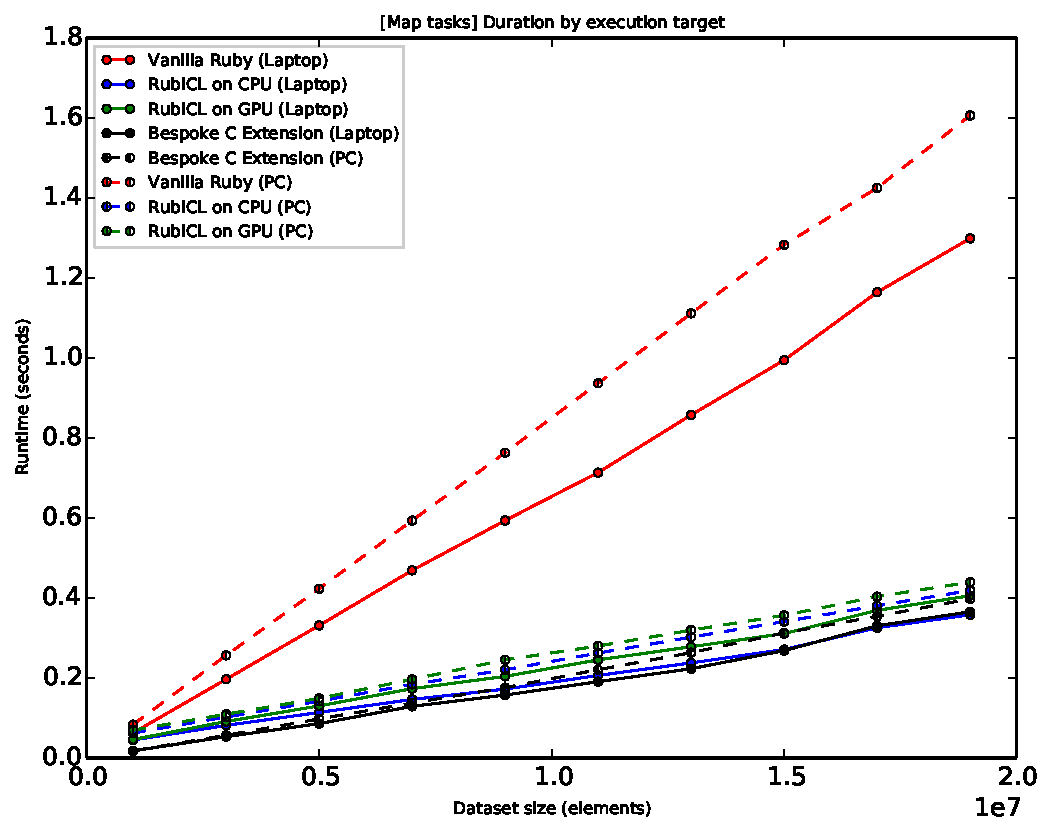
\includegraphics[width=\textwidth]{./graphing/just_map/runtimes.pdf}
  \caption{Task duration by execution target for \emph{Map}.}
  \label{fig:map_task_runtime_g}

\end{figure}
\begin{figure}[H]
  \centering

  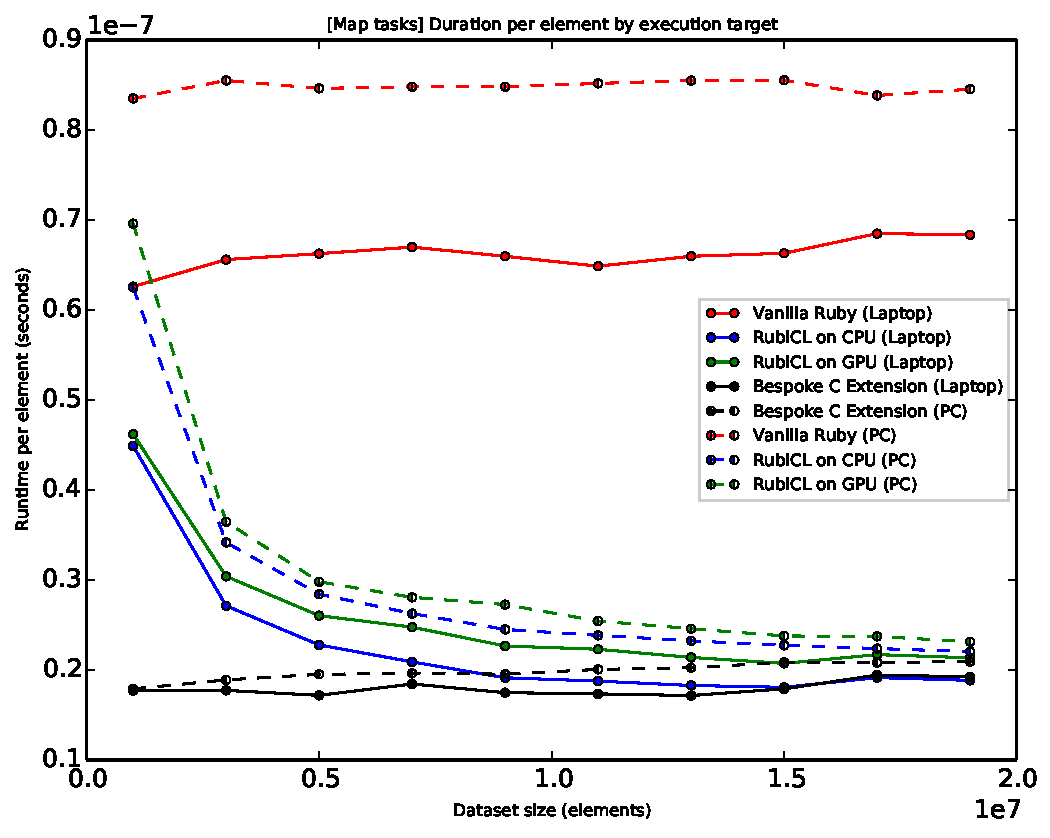
\includegraphics[width=\textwidth]{./graphing/just_map/per_element.pdf}
  \caption{Task duration per processed element for \emph{Map}.}
  \label{fig:map_task_per_el_g}

  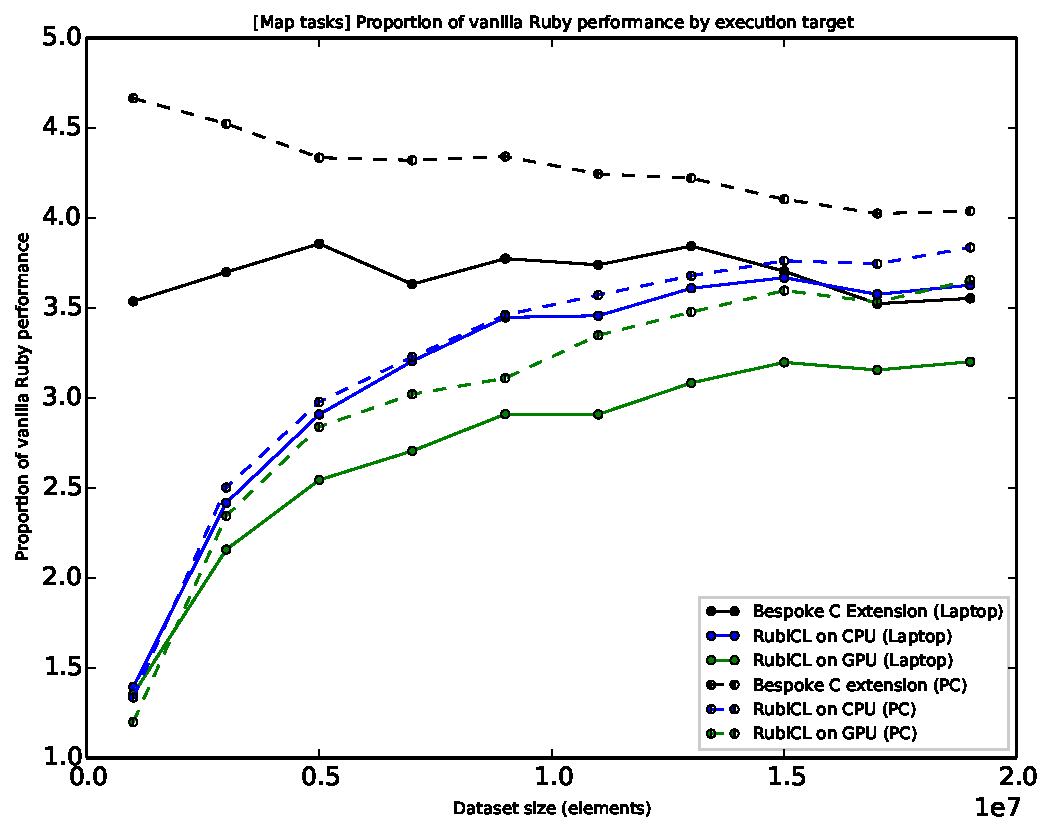
\includegraphics[width=\textwidth]{./graphing/just_map/prop_van.pdf}
  \caption{Proportion of vanilla Ruby performance achieved for \emph{Map}.}
  \label{fig:map_task_vperf_g}
\end{figure}
\begin{figure}[H]

  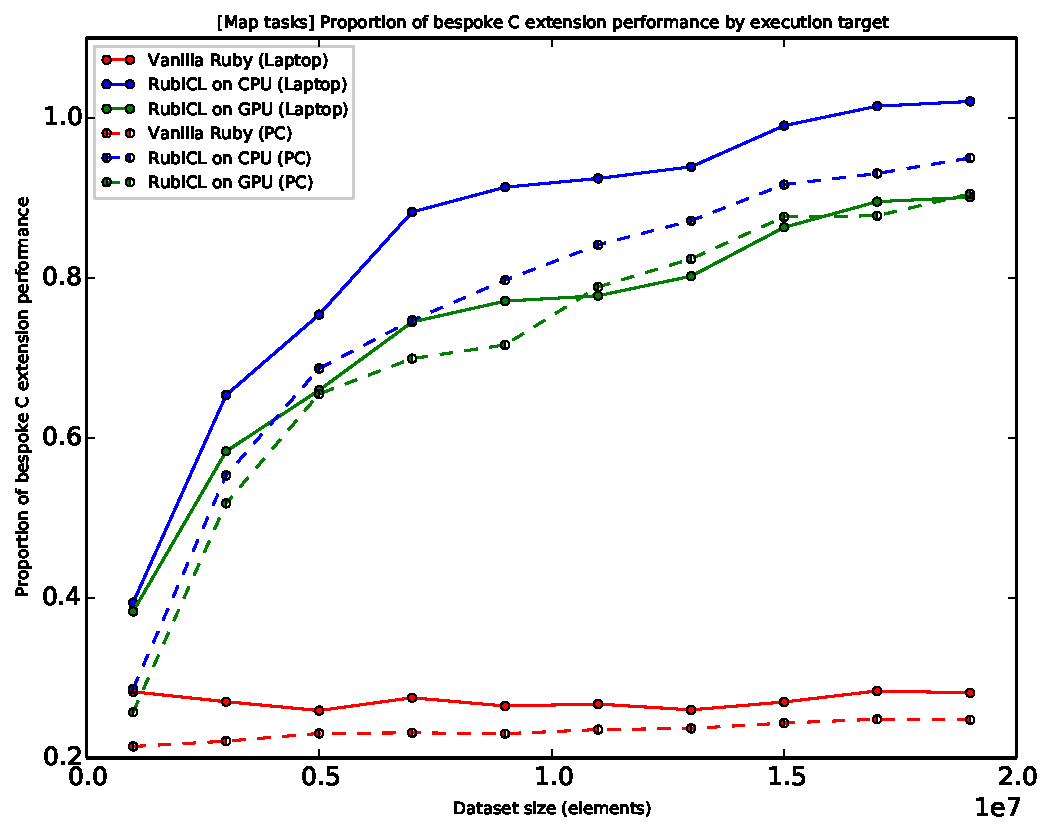
\includegraphics[width=\textwidth]{./graphing/just_map/prop_bes.pdf}
  \caption{Proportion of bespoke C extension performance achieved for \emph{Map}.}
  \label{fig:map_task_bperf_g}
\end{figure}
\paragraph*{Recap of operation performed}
The \emph{Map} task performed was the equivalent of \verb!#map { |x| x + 1 }!. This has the effect of incrementing every member of the input dataset.
Performing little work in the supplied function body produces a worst-case evaluation of library performance. This is because performing more work will allow increased throughput to mask any increased latency that the system has. Many tasks will be more involved than incrementation, and very few less so. A result showing that the library is beneficial here should apply even more to tasks that are of greater intensity.

\paragraph*{Observations and analysis}
Figure~\ref{fig:map_task_runtime_g} shows that all trialled alternatives exhibit similar performance when executing \emph{Map} tasks.
This is likely due to the computational simplicity of the task. The probable cause for the bottleneck is the need to move data in and out of the RubyVM's internal array structures.
Although the gap is slight, the \ac{CPU} compute-devices installed in both machines outperform the \acp{GPU} over the range of tested datasets. This is easiest to observe in Figure~\ref{fig:map_task_per_el_g}.

When parallelising purely-map tasks, the project library performs favourably compared to the standard \verb|Enumerable#map| implementation of Ruby $2.2$. Figure~\ref{fig:map_task_vperf_g} demonstrates that, at best, a factor $3.5$\textendash$4$ speed-up over typical execution can be achieved on both systems.
The figure also shows that for all tested datasets, the smallest of which contained $1$ million elements, outsourcing computation to the library was beneficial.

In Figure~\ref{fig:map_task_bperf_g}, it can be seen that on both systems RubiCL throughput is not far from bespoke sequential code. On the laptop, the parallel \ac{CPU} implementation exceeds the non-parallel native extension. It achieves $1.02$ times the rate of processing on $19$ million elements.
However, while the laptop \ac{CPU} presents $4$ hardware threads to \ac{OpenCL}, the native extension utilises only a single thread of execution. As both implementations are performing roughly the same number of operations, it appears that \ac{OpenCL}'s raw throughput increase is insignificant after the processing-model overhead is accounted for.

It is clear that the throughput with which Ruby is capable of performing \emph{Map} tasks has been significantly increased.
On the other hand, the project's parallel library does not significantly outperform a custom, tailored, sequential solution.
Yet, for all systems choosing the optimal device, no less than $80\%$ of the best-presented throughput is achieved at $10$ million elements, improving to no less than $95\%$ at $19$ million.
With the library providing automatic translation of all functions stated into parallel execution patterns, this deficit is insignificant. Much more significant is the mitigation of the need to write and compile native extensions for every required calculation.

\paragraph*{Smaller scale Map tasks}
\begin{figure}
  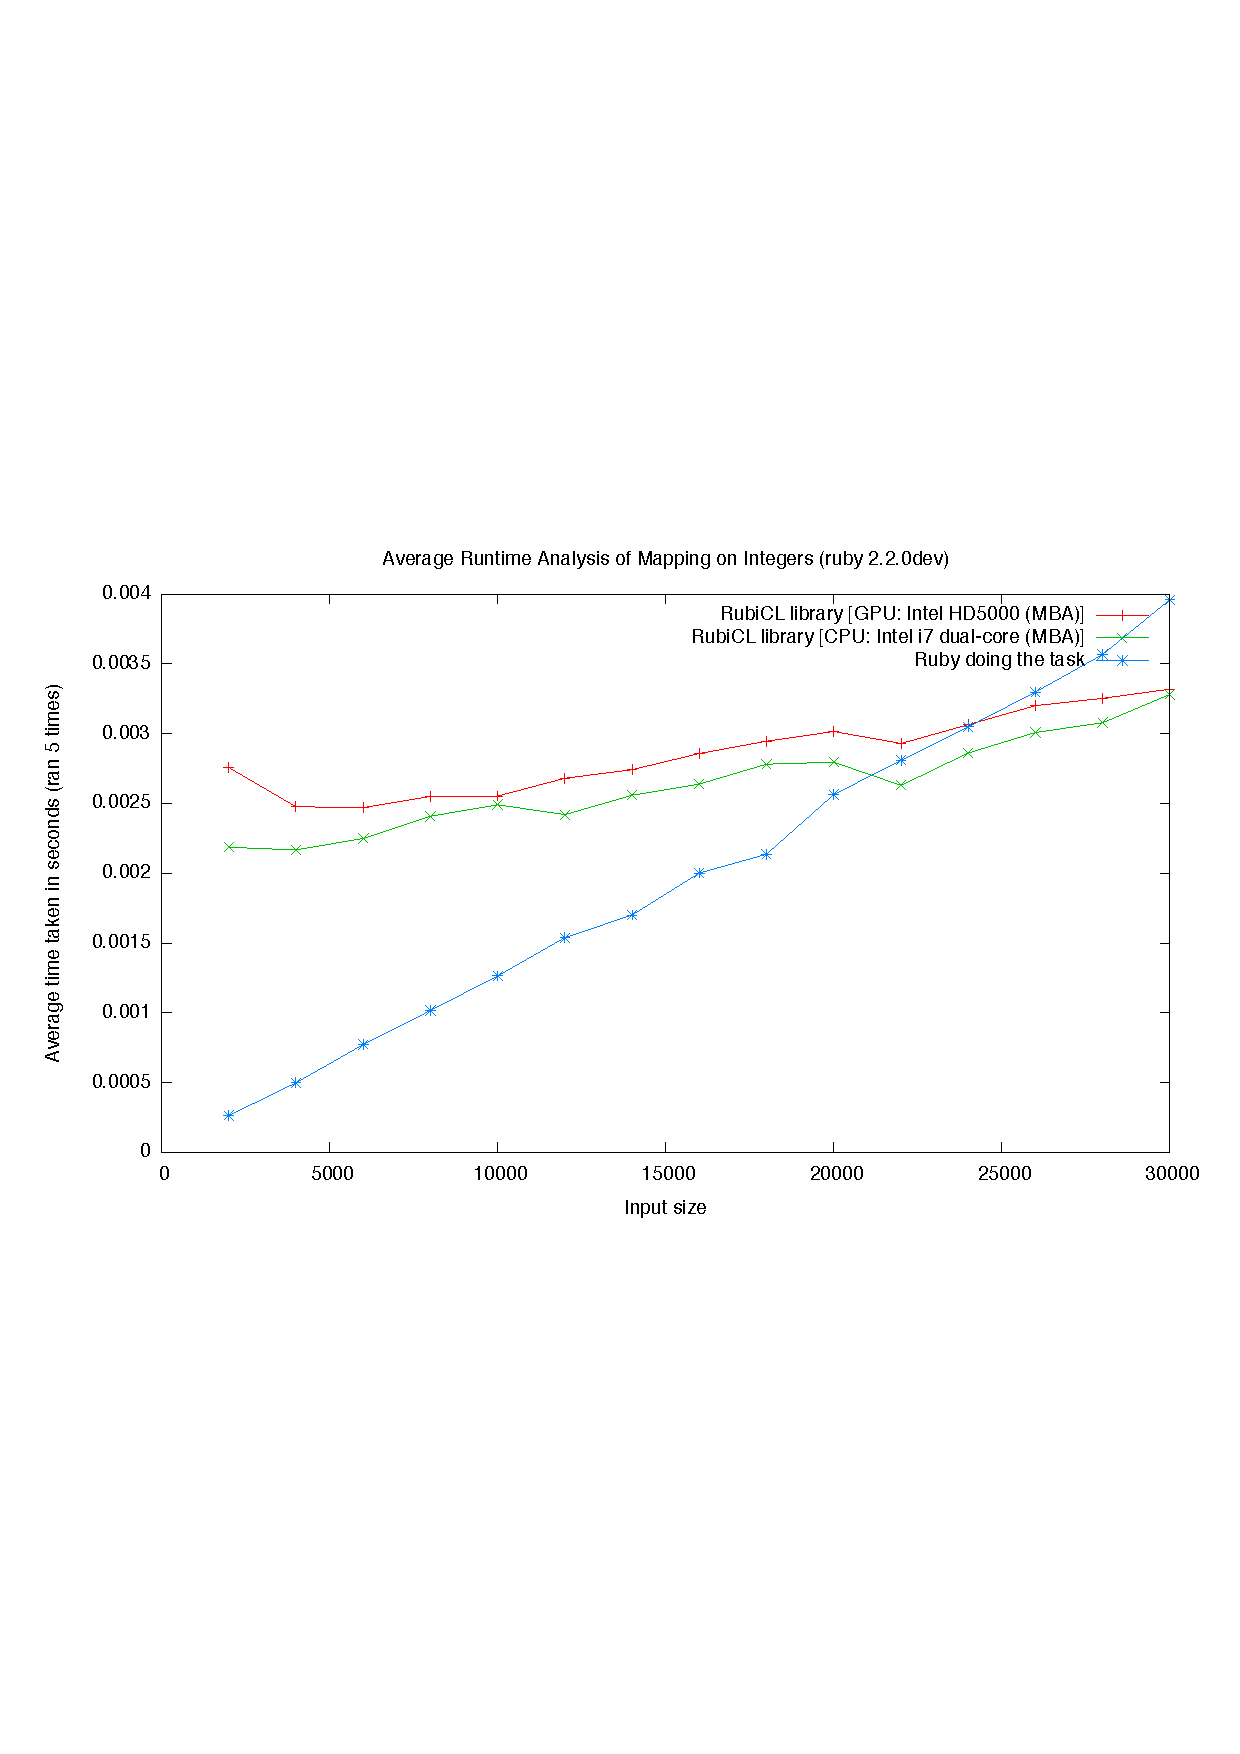
\includegraphics[trim=0cm 8cm 0cm 8cm, clip=true, width=\textwidth]{./graphing/smallmap.pdf}
  \caption{Duration for smaller-scale \emph{Map} tasks.}
  \label{fig:map_tasksmallrun}
\end{figure}

Figure~\ref{fig:map_tasksmallrun} shows that the RubiCL library, when executing on the laptop system, is beneficial for \emph{Map} tasks containing greater than $20,000$\textendash$25,000$ elements. It also demonstrates that the laptop system experiences task latency of around $20$ms.

\subsubsection{Floating-point performance}
\begin{figure}
  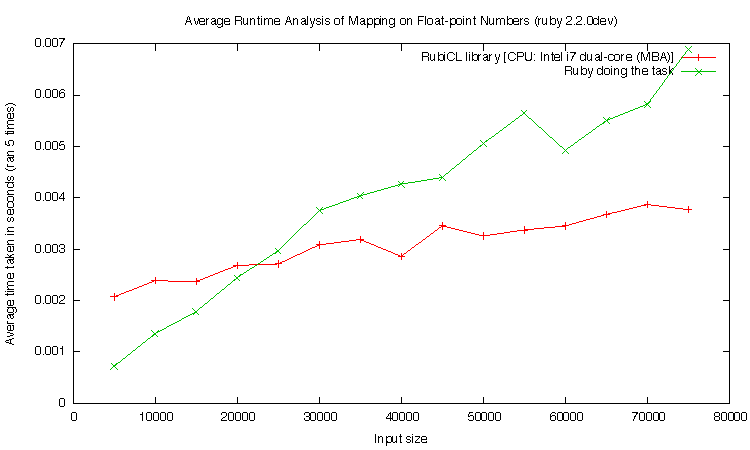
\includegraphics[width=\textwidth]{./graphing/smalldmap.pdf}
  \caption{Duration for smaller-scale \emph{Map} tasks on floating-point numbers}
  \label{fig:dmap_task_smallrun}
\end{figure}

\begin{figure}
  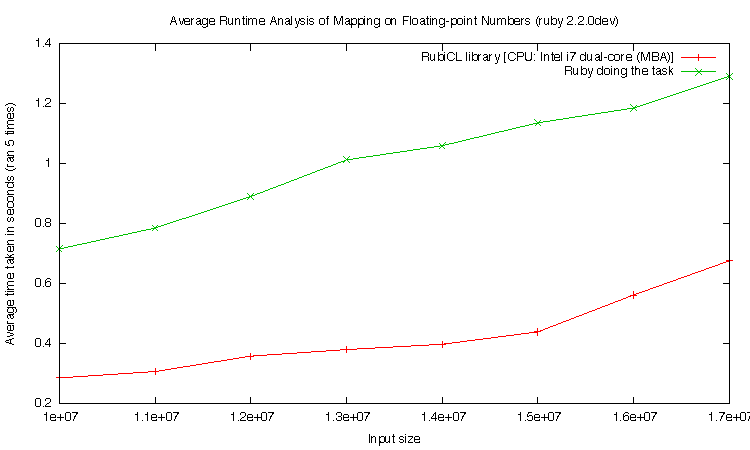
\includegraphics[width=\textwidth]{./graphing/dmaplarge.pdf}
  \caption{Duration for larger-scale \emph{Map} tasks on floating-point numbers}
  \label{fig:dmap_task_smallrun}
\end{figure}

Figure~\ref{fig:dmap_task_smallrun} shows that the lower-bound for beneficial \emph{Map} acceleration by the RubiCL library remains roughly the same for floating-point datasets as what was observed for integer datasets. Again, comparing \ac{OpenCL} execution on the \ac{CPU} to standard Ruby, it is worth outsourcing computation above $20,000$ elements.

The RubiCL library offers a speed-up of around $2$ times the traditional implementation. The reduction over integer speed-up is likely due to object conversion no longer occurring in parallel, and the linear dereference cost added to both implementations.


\subsection{Dense Filter tasks}
\subsubsection{Integer performance}
\begin{figure}[H]
  \centering
  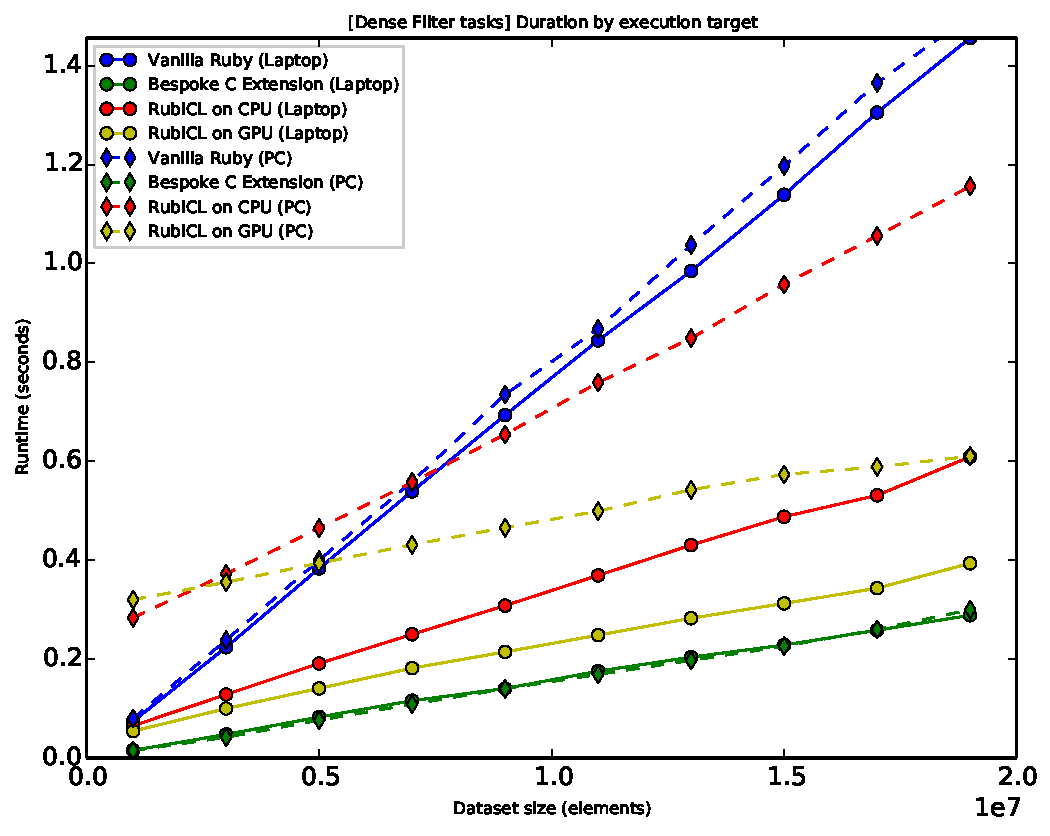
\includegraphics[width=\textwidth]{./graphing/dense_filter/runtimes.pdf}
  \caption{Task duration by execution target for dense \emph{Filter}.}
  \label{fig:dfilter_task_runtime_g}

  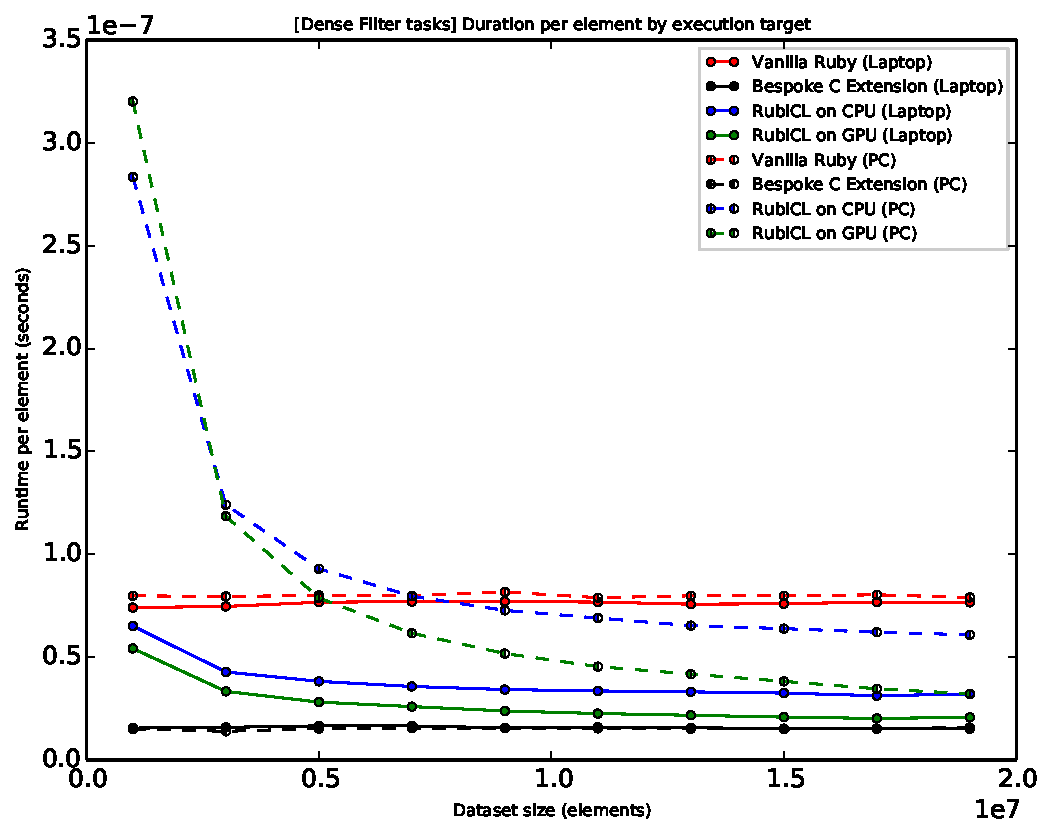
\includegraphics[width=\textwidth]{./graphing/dense_filter/per_element.pdf}
  \caption{Task duration per processed element for dense \emph{Filter}.}
  \label{fig:dfilter_task_per_el_g}

\end{figure}

\begin{figure}[H]
  \centering
  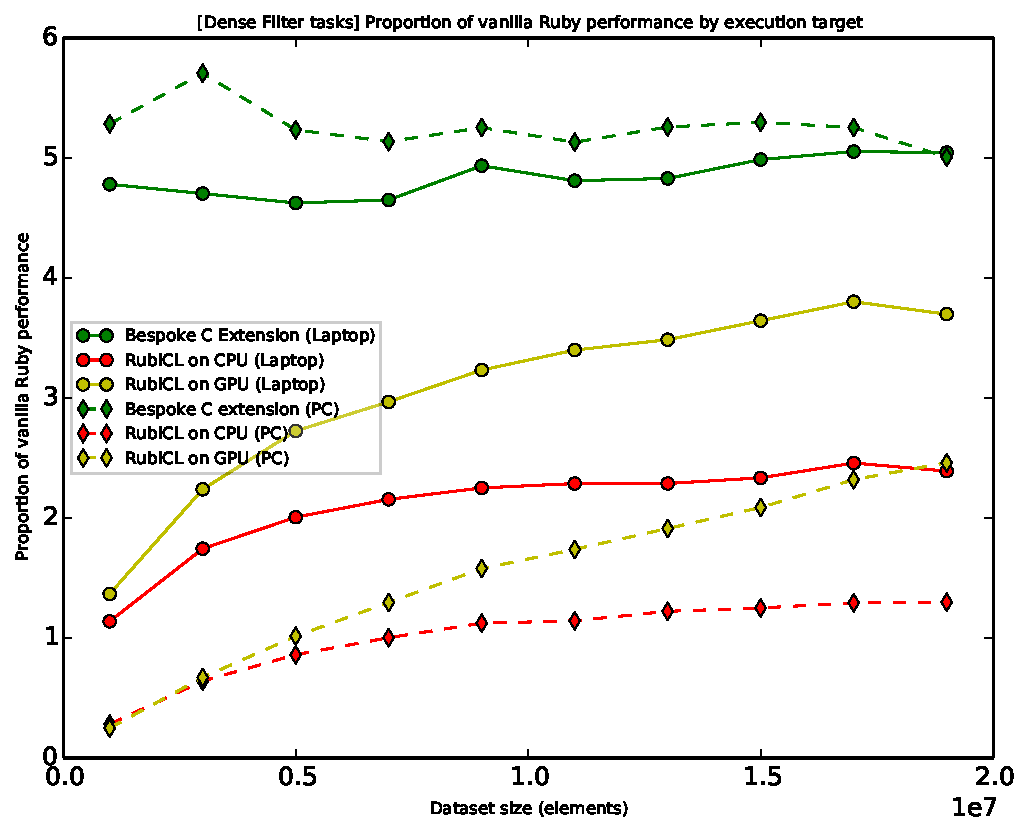
\includegraphics[width=\textwidth]{./graphing/dense_filter/prop_van.pdf}
  \caption{Proportion of vanilla Ruby performance achieved for dense \emph{Filter}.}
  \label{fig:dfilter_task_vperf_g}

  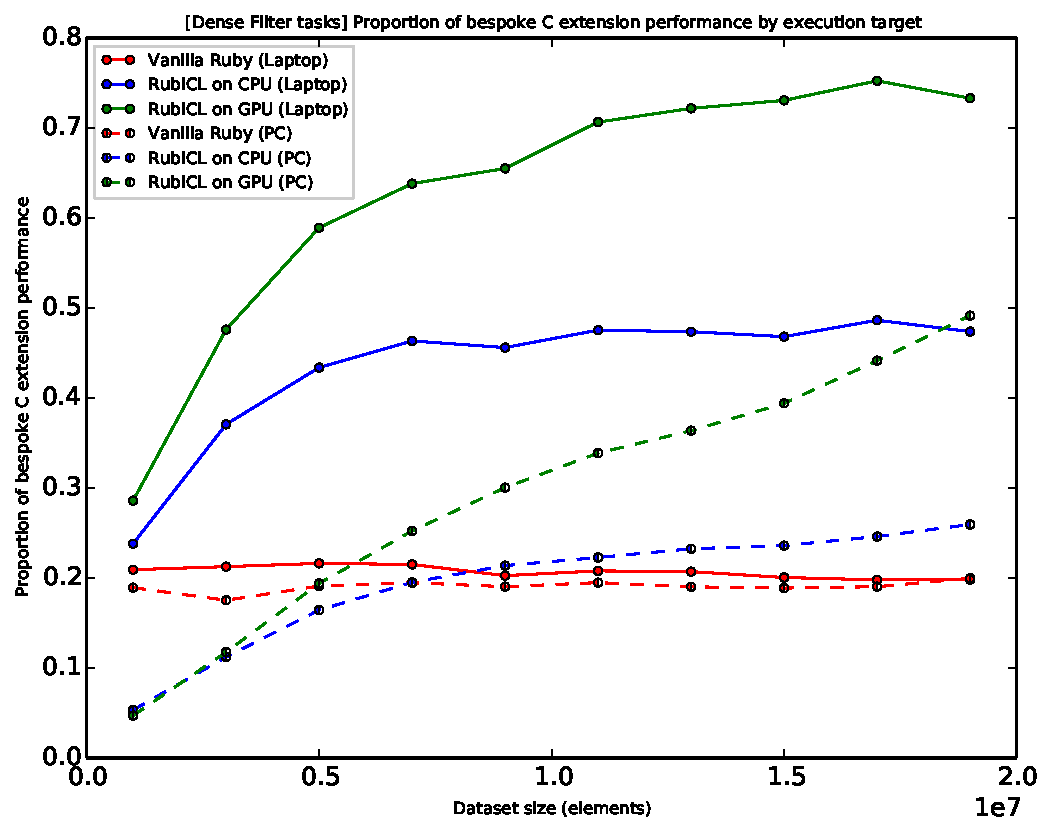
\includegraphics[width=\textwidth]{./graphing/dense_filter/prop_bes.pdf}
  \caption{Proportion of bespoke C extension performance achieved for dense \emph{Filter}.}
  \label{fig:dfilter_task_bperf_g}
\end{figure}
\paragraph*{Recap of operation performed}
The dense \emph{Filter} task performed was the equivalent of \verb!#select { |x| x.even? }!. With the ascending range of data supplied, this will return a subset of the input dataset with half the number of elements remaining.

\paragraph*{Observations and analysis}
Figure~\ref{fig:dfilter_task_runtime_g} is less cluttered than the corresponding graph for \emph{Map} tasks, as there is more variation between the performance of dense \emph{Filter} implementations.
The figure suggests that \emph{Filter} tasks scheduled on the desktop system suffer from a higher latency than their counterparts on the laptop. This is signified by the comparatively elevated runtime for smaller datasets.

Further unlike \emph{Map} tasks, on both systems the \ac{GPU} compute-devices outperform the \ac{CPU} when filtering large datasets. For the laptop system, the domination is present on every tested dataset size. On the contrary, the desktop \ac{CPU} is initially a shade faster but is quickly dwarfed by the significantly higher throughput of the \ac{GPU} device.

On the laptop system, Figure~\ref{fig:dfilter_task_vperf_g} demonstrates that the library is beneficial when processing all datasets within the tested range. The desktop is not quite as successful at performing dense purely-\emph{Filter} tasks, hampered when producing subsets of smaller datasets by its increased latency. At least $5$ million elements are required before it is worthwhile to offload computation onto the \ac{GPU} via RubiCL. The \ac{CPU} trails not long after, at $8$ million elements, but never achieves more than $25\%$ speed-up over the standard Ruby implementation.

On both test systems, when using the \ac{GPU}, a noticeable speed-up of \emph{Filter} operations can be achieved. With a $2.5$ times speed-up on the desktop and over $3.5$ times on the laptop, large filtering operations are significantly accelerated by the RubiCL library.

Figure~\ref{fig:dfilter_task_bperf_g} shows that the laptop \ac{GPU} achieves a high proportion, peaking at $75\%$, of bespoke sequential code performance. The desktop system boasts a lesser proportion, at $50\%$, but the lack of plateau in the figure suggests that this gap would close further as datasets increase in size.

The lacklustre performance when executing on \ac{CPU} devices can be partly explained by the fact that the parallel implementation of filtering, although asymptotically identical in cost, requires much more work than a sequential filter. In this case, the hidden constants involved for distributing computation have a large effect on the task duration, larger than that of parallelising the predicate scan and index calculations along the data.

This reasoning can also explain why the \ac{GPU} devices fail to outperform the custom extension over the given range of datasets.
Nonetheless, the need to write and compile native extensions for each distinct query performed is again removed when using the RubiCL library. A system-dependent performance hit of between $25\%$ and $50\%$ behind a handwritten extension is far more justifiable when it facilitates rapid-prototyping, especially when compared to the $80\%$ penalty that Figure~\ref{fig:dfilter_task_bperf_g} highlights for unoptimised Ruby $2.2$.

\paragraph*{Smaller scale dense Filter tasks}
\begin{figure}[H]
  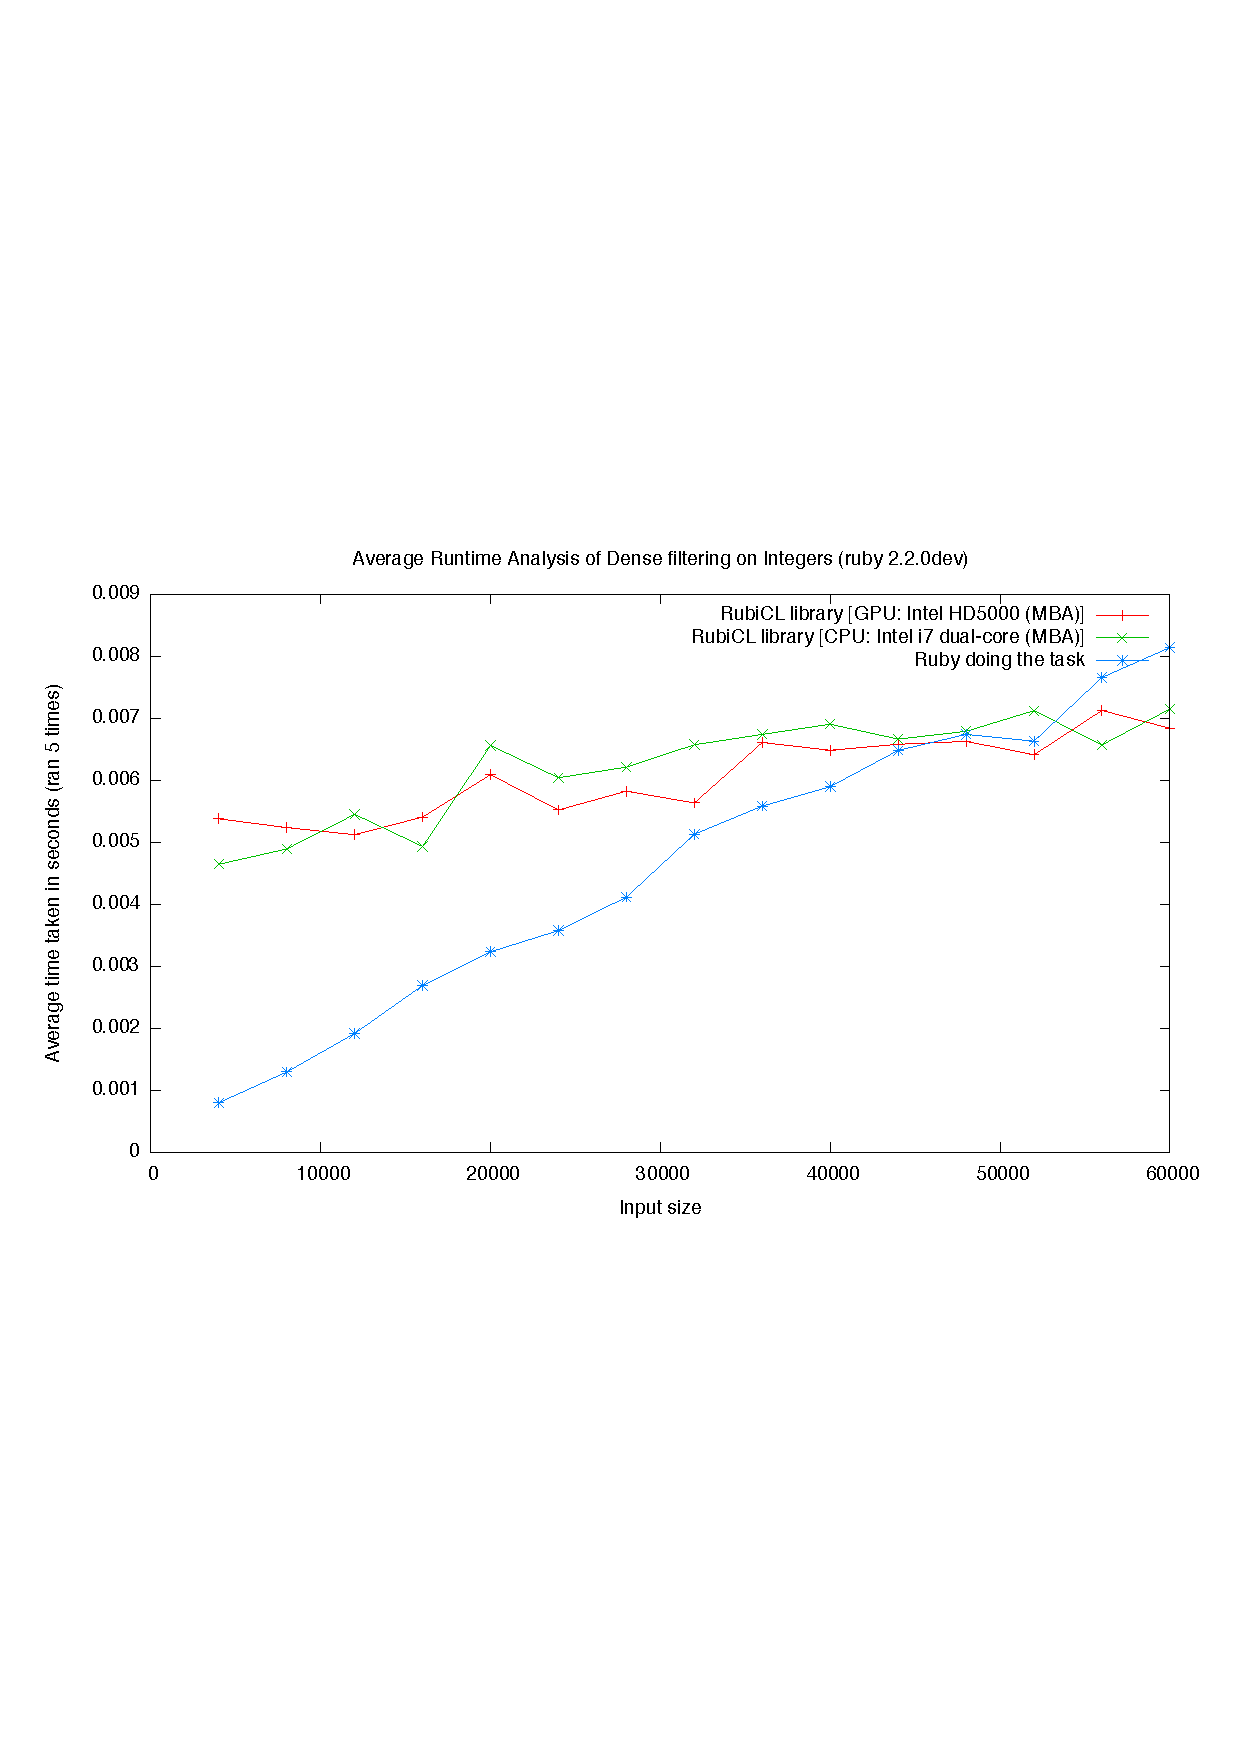
\includegraphics[trim=0cm 8cm 0cm 8cm, clip=true, width=\textwidth]{./graphing/smalldensefilter.pdf}
  \caption{Duration for smaller-scale dense \emph{Filter} tasks.}
  \label{fig:densefil_tasksmallrun}
\end{figure}
Figure~\ref{fig:densefil_tasksmallrun} shows that the RubiCL library, when executing on the laptop system, is beneficial for dense \emph{Filter} tasks containing greater than $50,000$ elements. It also demonstrates that the laptop system experiences task latency of around $50$ms.

\subsubsection{Floating-point performance}
\begin{figure}
  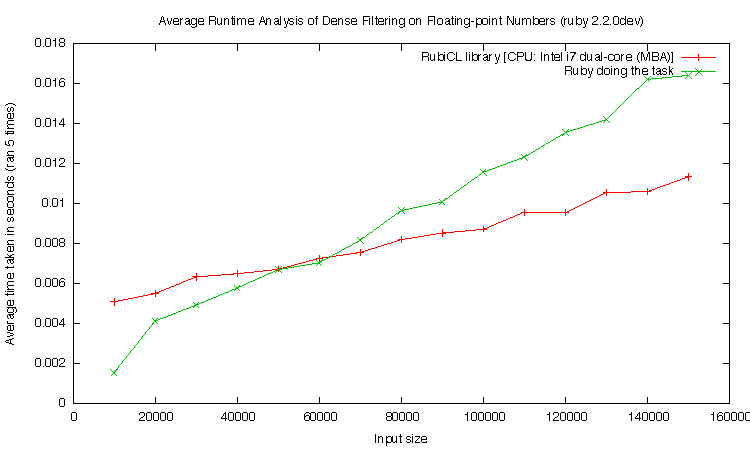
\includegraphics[width=\textwidth]{./graphing/ddensefilter.pdf}
  \caption{Duration for smaller-scale dense \emph{Filter} tasks on floating-point numbers}
  \label{fig:dddf_task_smallrun}
\end{figure}

\begin{figure}
  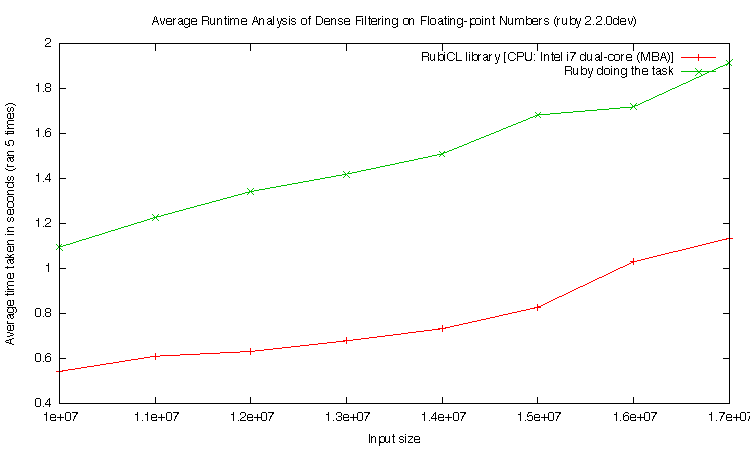
\includegraphics[width=\textwidth]{./graphing/ddfilterlots.pdf}
  \caption{Duration for larger-scale dense \emph{Filter} tasks on floating-point numbers}
  \label{fig:dddf_task_bigrun}
\end{figure}

Figure~\ref{fig:dddf_task_smallrun} shows that the lower-bound for beneficial dense \emph{Filter} acceleration by the RubiCL library remains roughly the same for floating-point datasets as what was observed for integer datasets. Again, comparing \ac{OpenCL} execution on the \ac{CPU} to standard Ruby, it is worth outsourcing computation above $50,000$ elements.

The RubiCL library offers a speed-up of around $2$ times the traditional implementation. This is shown in Figure~\ref{fig:dddf_task_bigrun} and is nearly identical to the \ac{CPU} speed-up achieved for integer datasets. This suggests that the added cost of object dereferencing and re-creation, necessary for all implementations, is insignificant compared to the work involved when performing a filtering operation.


\subsection{Sparse Filter tasks}
\subsubsection{Integer performance}
\begin{figure}[H]
  \centering
  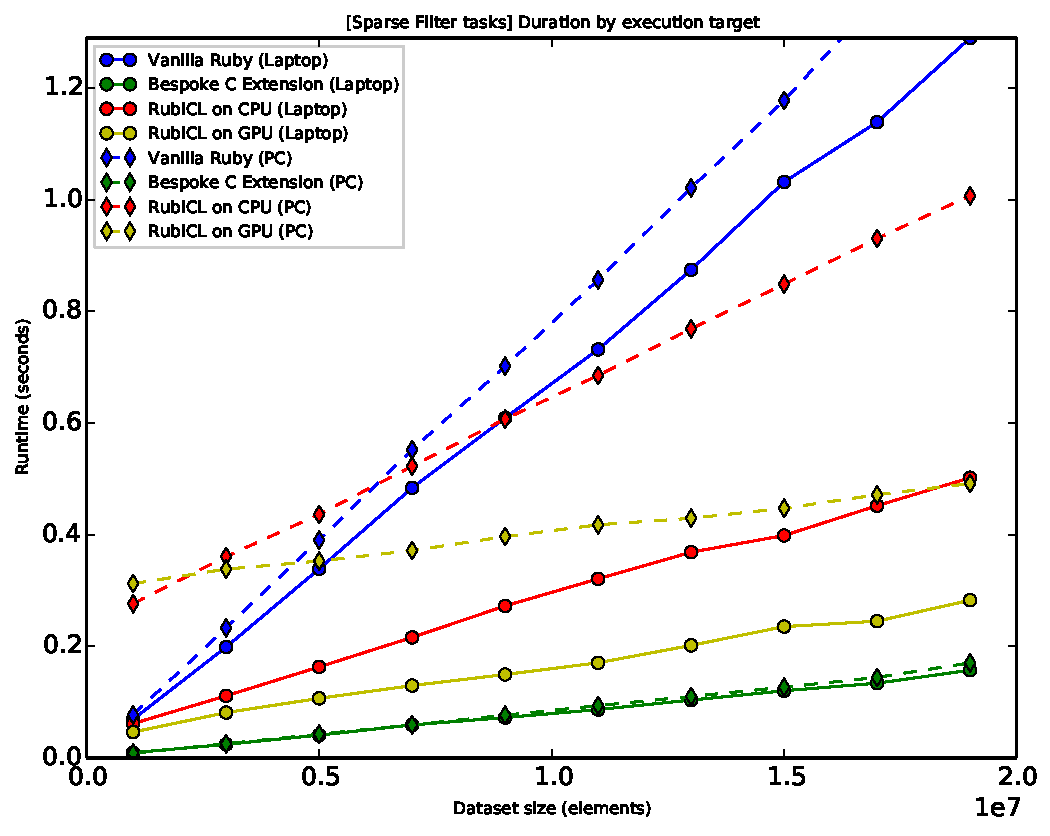
\includegraphics[width=\textwidth]{./graphing/sparse_filter/runtimes.pdf}
  \caption{Task duration by execution target for sparse \emph{Filter}.}
  \label{fig:sfilter_task_runtime_g}

  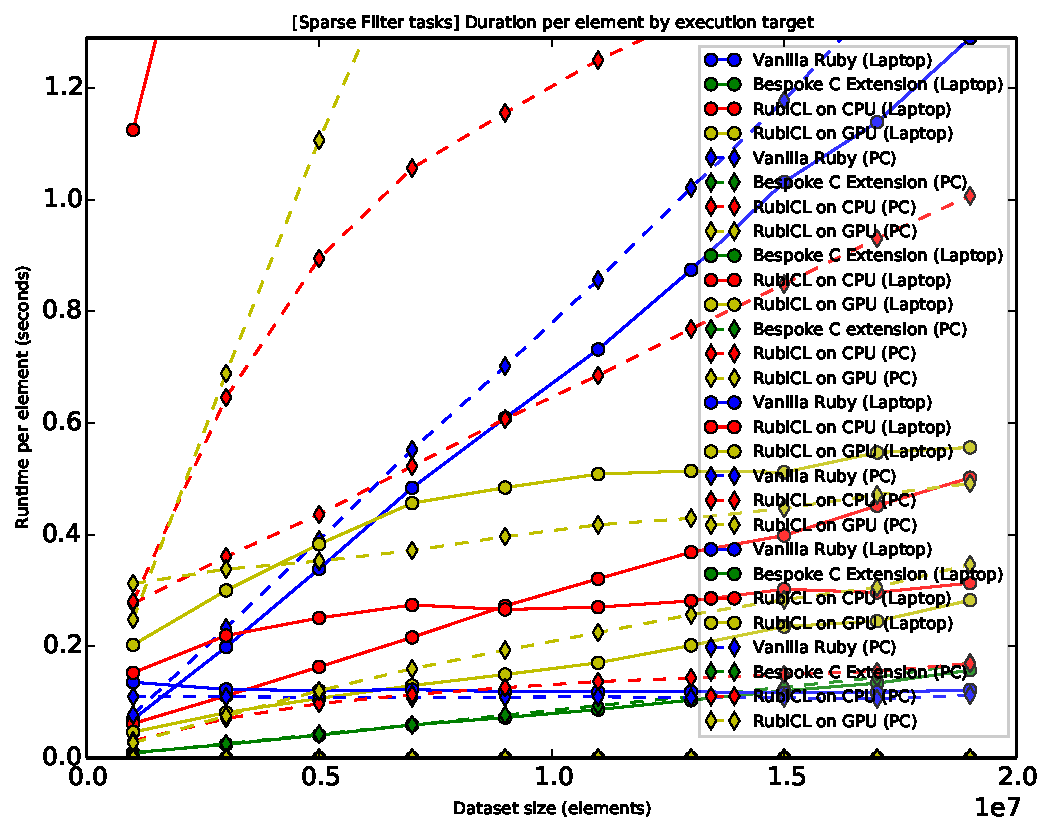
\includegraphics[width=\textwidth]{./graphing/sparse_filter/per_element.pdf}
  \caption{Task duration per processed element for sparse \emph{Filter}.}
  \label{fig:sfilter_task_per_el_g}

\end{figure}

\begin{figure}[H]
  \centering
  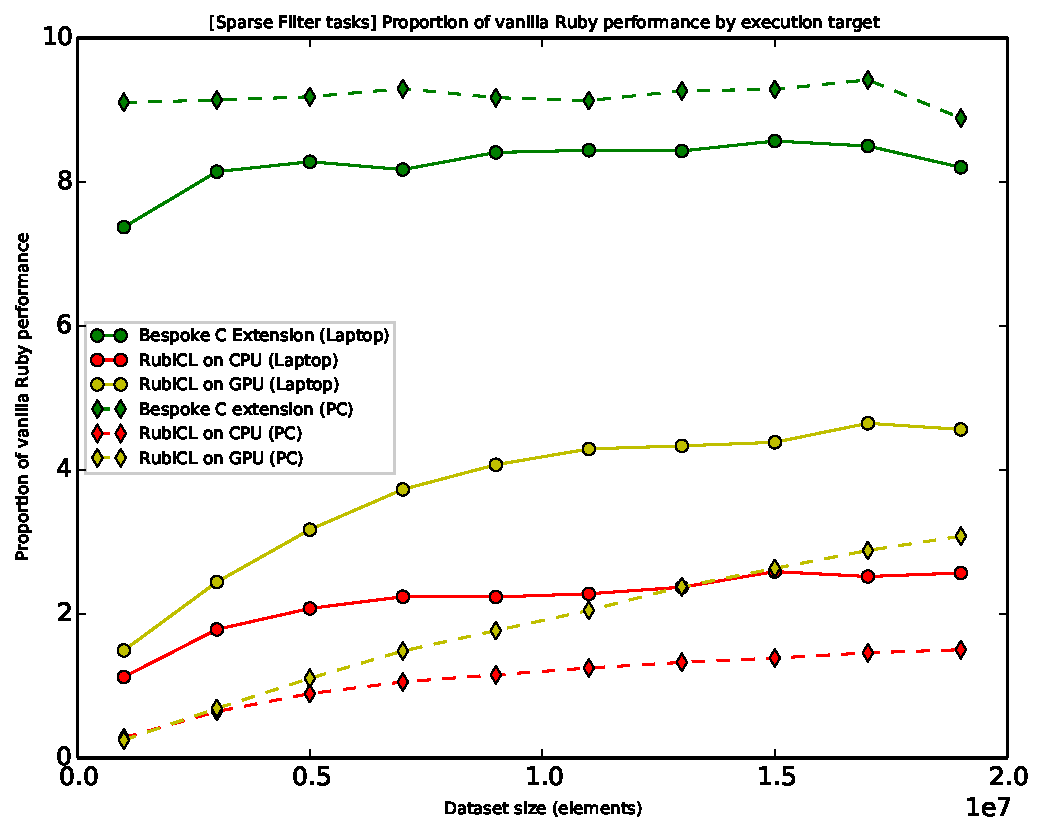
\includegraphics[width=\textwidth]{./graphing/sparse_filter/prop_van.pdf}
  \caption{Proportion of vanilla Ruby performance achieved for sparse \emph{Filter}.}
  \label{fig:sfilter_task_vperf_g}

  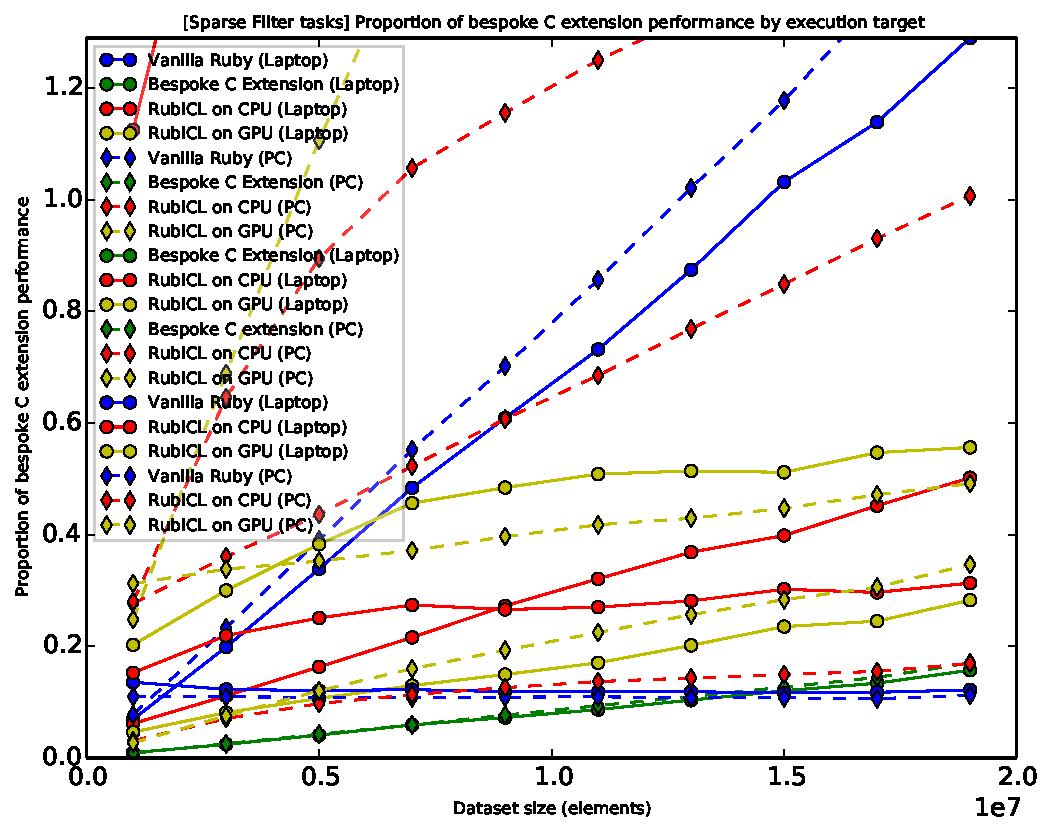
\includegraphics[width=\textwidth]{./graphing/sparse_filter/prop_bes.pdf}
  \caption{Proportion of bespoke C extension performance achieved for sparse \emph{Filter}.}
  \label{fig:sfilter_task_bperf_g}
\end{figure}
\paragraph*{Recap of operation performed}
The sparse \emph{Filter} task, returning fewer elements than the dense task, performed was the equivalent of \verb!#select { |x| x % 20 == 0 }!. This selects all elements that are evenly divisible by 20. With the ascending range of data supplied, this will return a subset of the input dataset with $5\%$ of its elements remaining.

\paragraph*{Observations and analysis}
Figure~\ref{fig:sfilter_task_runtime_g} looks very similar to that of dense filtering. Indeed, many of the observations are the same.
One reason for this is that none of the code benchmarked, including \verb|Enumerable#select|, changes behaviour when datasets are sparse.
Instead, the slight change in performance can be explained by differing proportions of time spent inserting elements or transferring device datasets when the set of returned results is smaller in size.

As before, the difference in latency between the laptop and desktop systems causes a significant proportional gap for smaller datasets.
It leaves sparse \emph{Filter} needing the same minimum dataset sizes for beneficial inclusion as dense \emph{Filter}.
This identical result is useful as it suggests that the threshold for parallelisation can be estimated without prior knowledge of the proportion of data retained.

Yet again, \ac{GPU} devices are dominant among the \ac{OpenCL} filtering implementations, for all but the smallest dataset on the desktop.
Much like the previous graph for filtering, the desktop \ac{GPU} does not appear to have plateaued in time-per-element. Therefore, further study should be performed to see at what size dataset this occurs.

The bespoke extension performs much better comparatively at sparse filtering than dense filtering. Figure~\ref{fig:sfilter_task_vperf_g} shows a $9$ times performance speed-up over unoptimised code, nearly twice the speed-up of dense filtering.
With this in mind, Figure~\ref{fig:sfilter_task_bperf_g} shows a decrease in performance of RubiCL relative to bespoke filtering, compared to the denser predicate examined earlier.

The inverse is true in Figure~\ref{fig:sfilter_task_vperf_g}, with RubiCL demonstrating an improved $3$\textendash$5$ times speed-up when executing on \ac{GPU} devices over Ruby $2.2$ for dense filtering.
The differences in relative performance between dense and sparse \emph{Filter} task implementations suggest that the cause for diverging ratios may result from there being fewer conditional insertions to the result vector. Alternatively, when less data is returned from a compute-device, less time is spent, proportionally, in the comparatively slow operation of cross-device data transfer compared to the quick action of filtering itself.

\paragraph*{Smaller scale sparse Filter tasks}
\begin{figure}[H]
  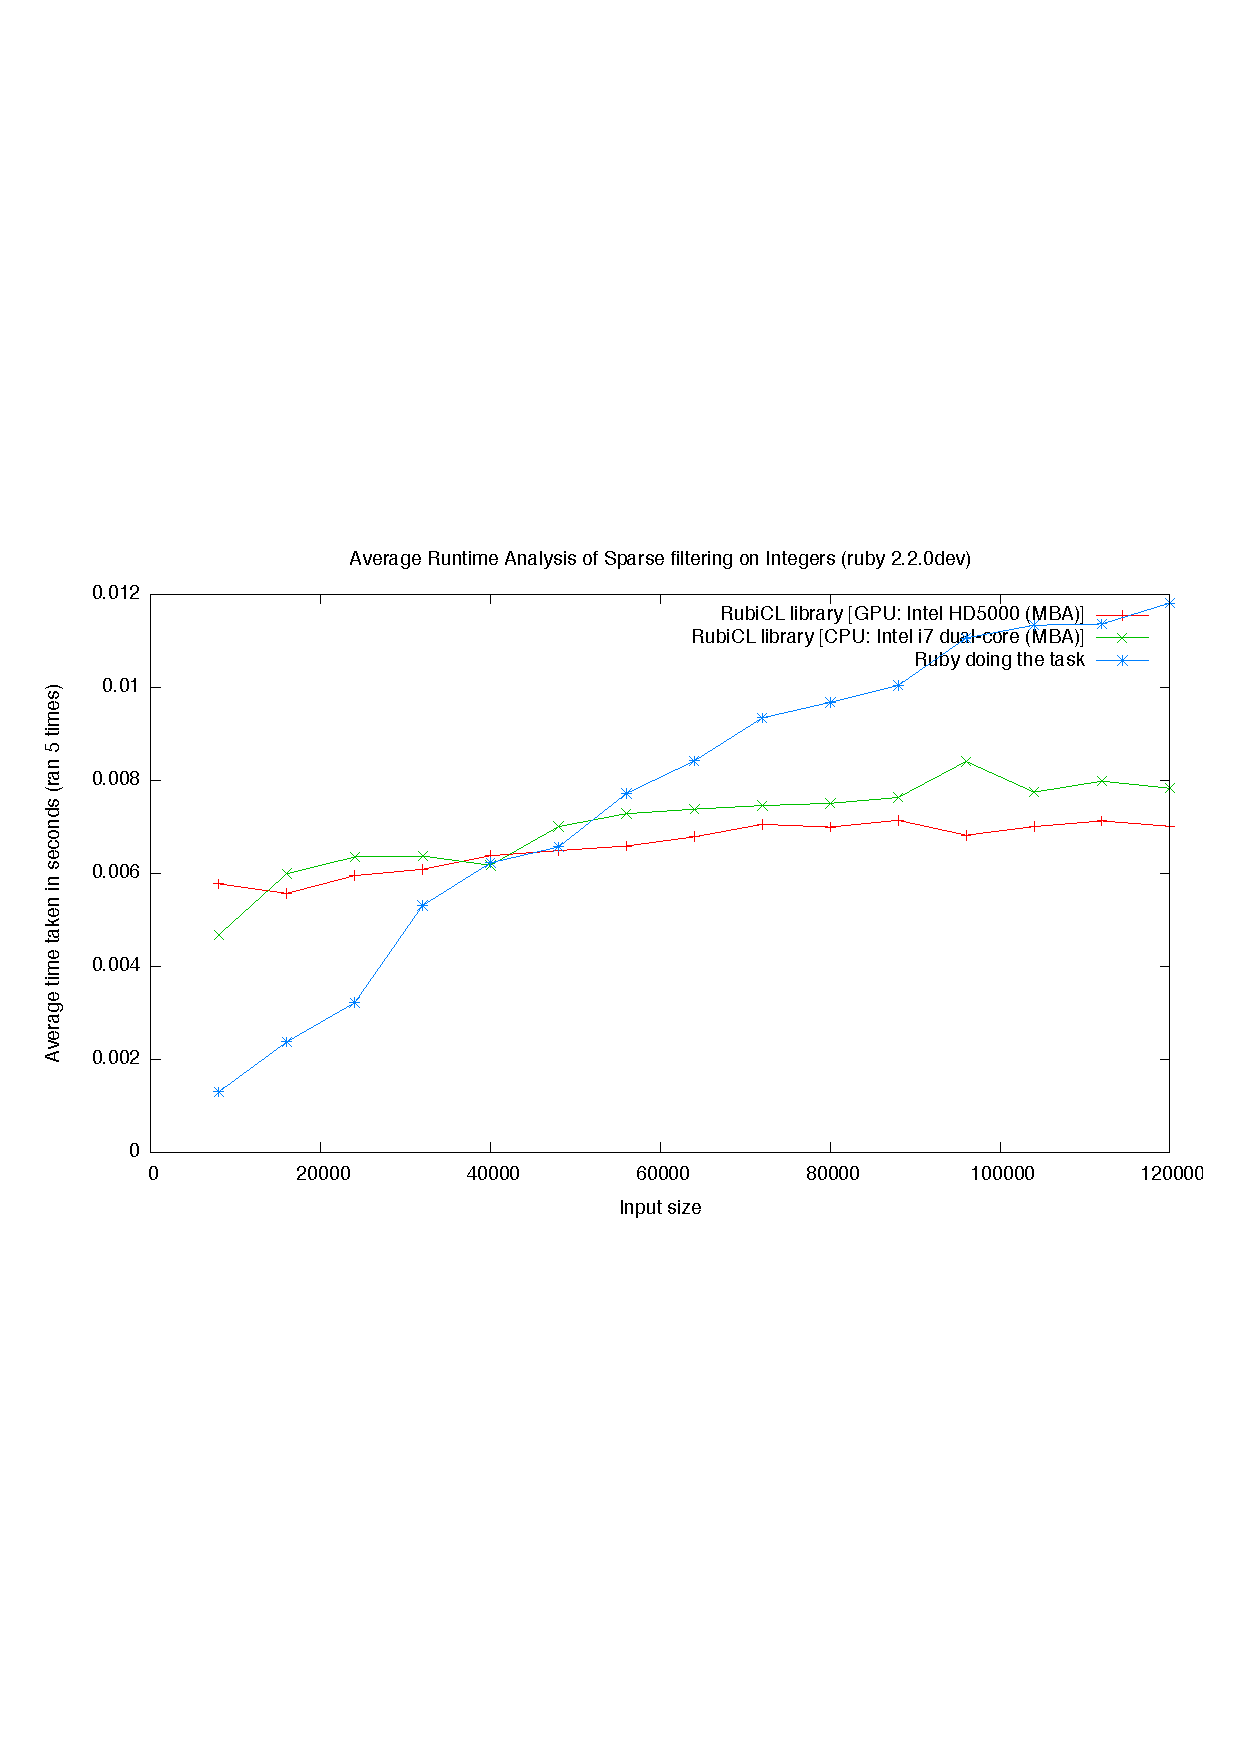
\includegraphics[trim=0cm 8cm 0cm 8cm, clip=true, width=\textwidth]{./graphing/smallsparsefilter.pdf}
  \caption{Duration for smaller-scale sparse \emph{Filter} tasks.}
  \label{fig:sparsefil_tasksmallrun}
\end{figure}
Figure~\ref{fig:sparsefil_tasksmallrun} shows that the RubiCL library, when executing on the laptop system, is beneficial for sparse \emph{Filter} tasks containing greater than $50,000$ elements. This is identical to the dense \emph{Filter} cutoff. It also demonstrates that the laptop system experiences task latency of around $50$ms.

\subsubsection{Floating-point performance}
\begin{figure}
  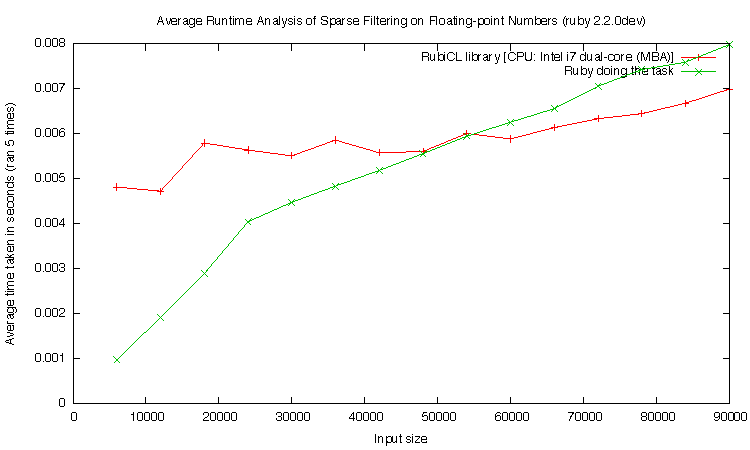
\includegraphics[width=\textwidth]{./graphing/dsparsesmall.pdf}
  \caption{Duration for smaller-scale sparse \emph{Filter} tasks on floating-point numbers}
  \label{fig:dsdf_task_smallrun}
\end{figure}

\begin{figure}
  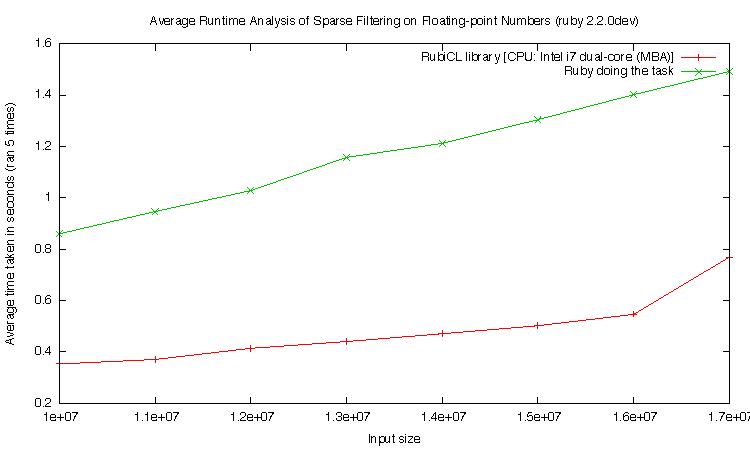
\includegraphics[width=\textwidth]{./graphing/dsfilterlots.pdf}
  \caption{Duration for larger-scale sparse \emph{Filter} tasks on floating-point numbers}
  \label{fig:dsdf_task_bigrun}
\end{figure}

Figure~\ref{fig:dsdf_task_smallrun} shows that the lower-bound for beneficial sparse \emph{Filter} acceleration by the RubiCL library remains roughly the same for floating-point datasets as what was observed for integer datasets. Again, comparing \ac{OpenCL} execution on the \ac{CPU} to standard Ruby, it is worth outsourcing computation above $50,000$ elements.

Figure~\ref{fig:dsdf_task_bigrun} demonstrates that the RubiCL library offers a speed-up of around $2$ times the traditional implementation. Again, this is nearly identical to the \ac{CPU} speed-up achieved for integer datasets and suggests that the added cost of object dereferencing and re-creation, necessary for all implementations, is insignificant compared to the work involved when performing a filtering operation.



\subsection{MapFilter tasks}
\subsubsection{Integer performance}
\begin{figure}[H]
  \centering
  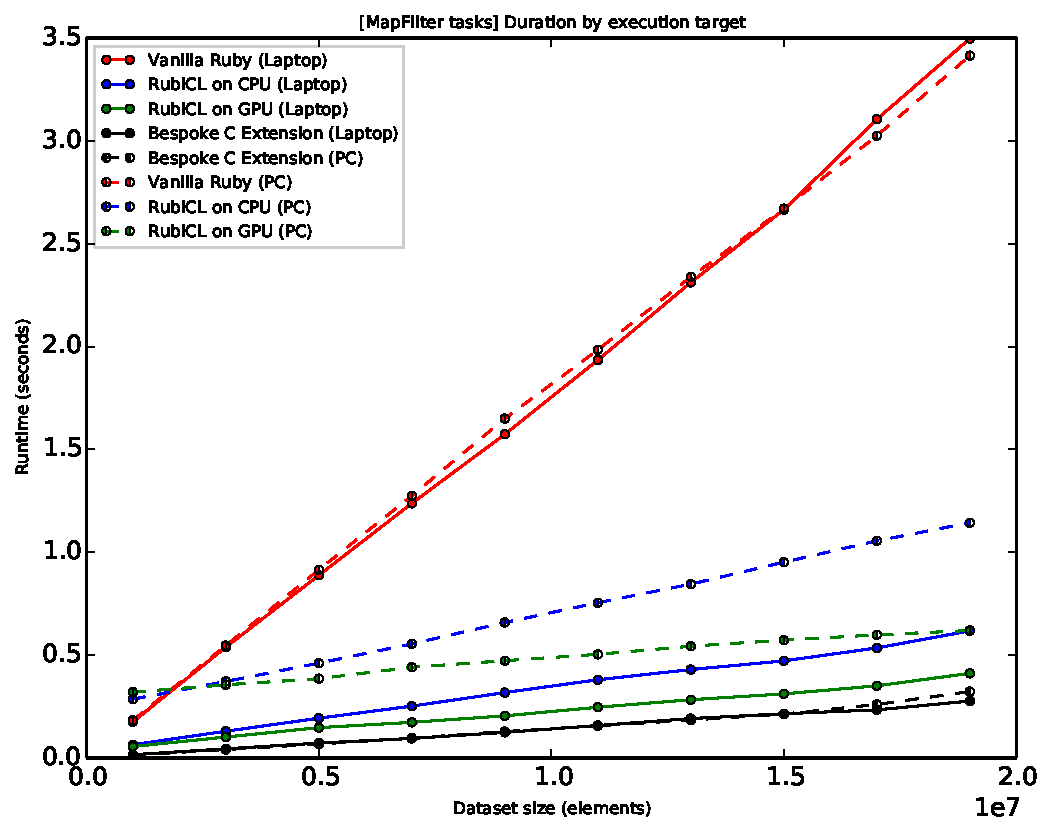
\includegraphics[width=\textwidth]{./graphing/mapfilter/runtimes.pdf}
  \caption{Task duration by execution target for \emph{MapFilter}.}
  \label{fig:mfilter_task_runtime_g}

  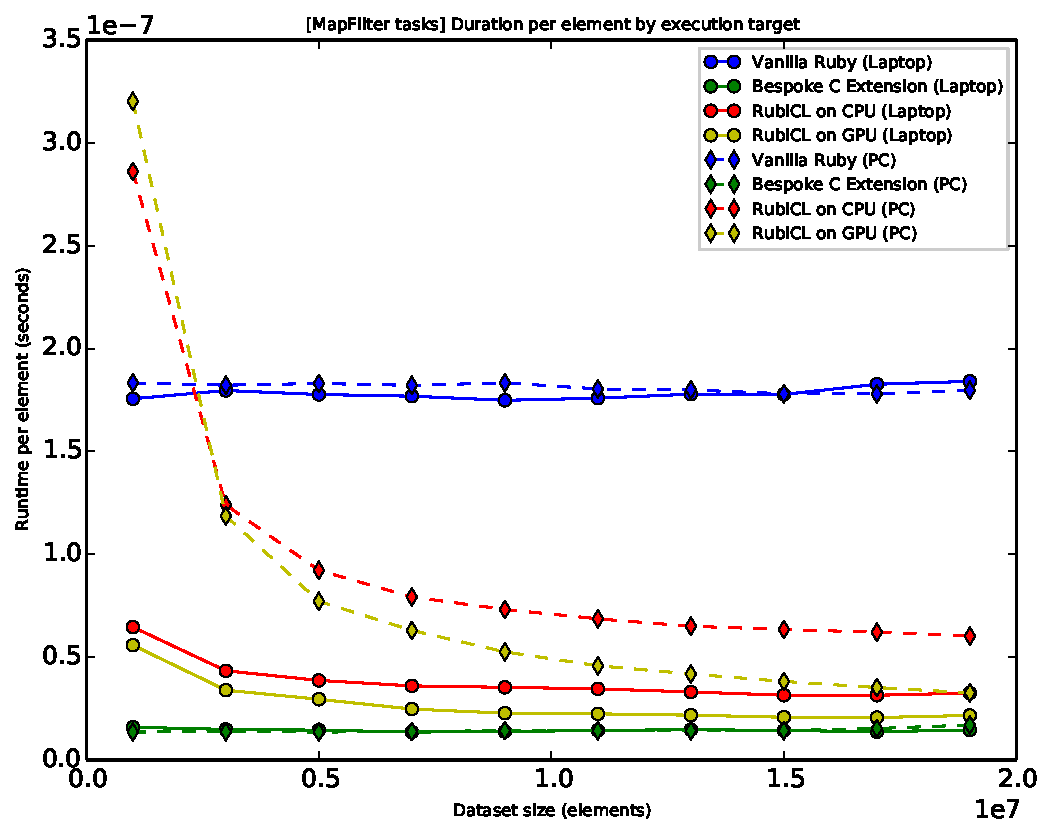
\includegraphics[width=\textwidth]{./graphing/mapfilter/per_element.pdf}
  \caption{Task duration per processed element for \emph{MapFilter}.}
  \label{fig:mfilter_task_per_el_g}

\end{figure}

\begin{figure}[H]
  \centering
  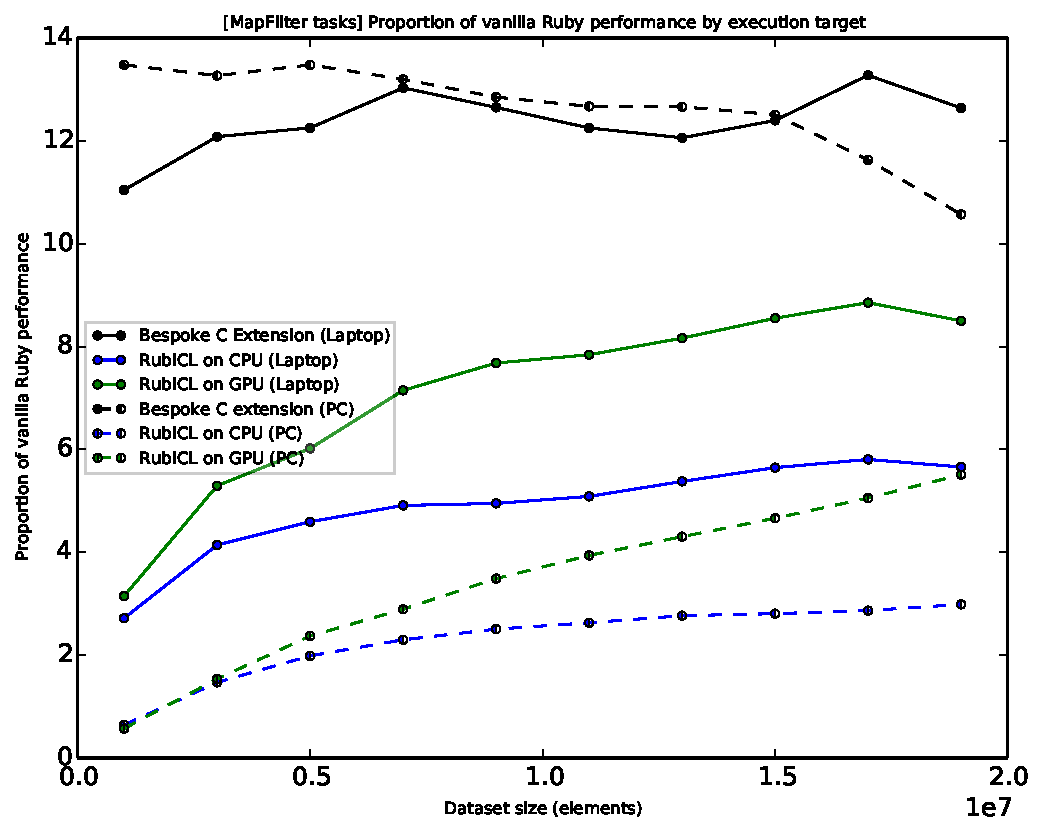
\includegraphics[width=\textwidth]{./graphing/mapfilter/prop_van.pdf}
  \caption{Proportion of vanilla Ruby performance achieved for \emph{MapFilter}.}
  \label{fig:mfilter_task_vperf_g}

  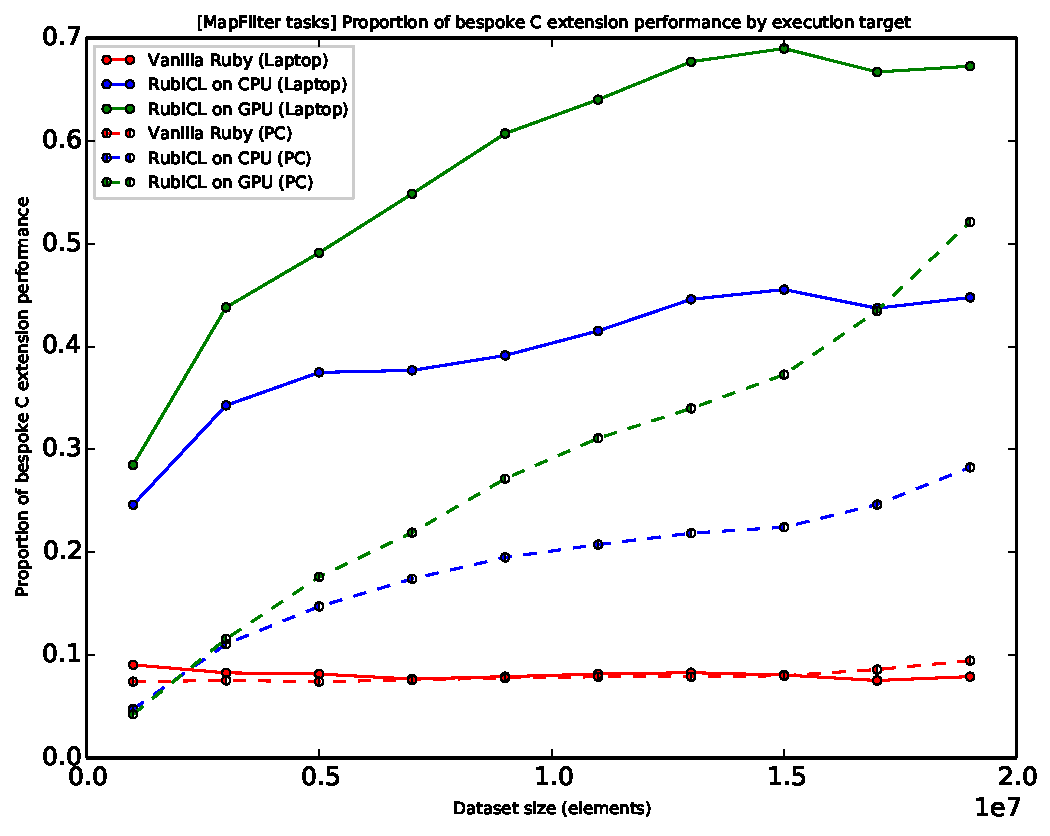
\includegraphics[width=\textwidth]{./graphing/mapfilter/prop_bes.pdf}
  \caption{Proportion of bespoke C extension performance achieved for \emph{MapFilter}.}
  \label{fig:mfilter_task_bperf_g}
\end{figure}
\paragraph*{Recap of operation performed}
The computation pipeline for this benchmark consisted of the earlier \emph{Map} task, immediately followed by the dense \emph{Filter} task.
This has the combined effect of incrementing all elements and then returning the subset of mutated elements that are even.
Again this returns a dataset that is half of the original size. Furthermore, the tasks can undergo \emph{fusion} in order to reduce the number of kernels scheduled and required passes over the data.


\paragraph*{Observations and analysis}
When a \emph{Map} task is followed by a \emph{Filter} task, the project's task fusion optimisation drastically improves performance.
Figure~\ref{fig:mfilter_task_runtime_g} demonstrates how significantly runtime diverges, with the gap between Ruby $2.2$ and competing implementations expanding greatly as larger datasets are introduced.
The need for multiple passes over the data greatly delays the unoptimised code, as intermediate yet discarded results for the method pipeline are computed.
The optimisation can be seen to reduce the minimum dataset length required for RubiCL's desktop parallelism to provide performance gains over the standard implementation, shown in Figure~\ref{fig:mfilter_task_vperf_g}. At just $2$ million elements, it is less than half of that required when filtering alone.

Figure~\ref{fig:mfilter_task_vperf_g} also demonstrates the significant throughput increases provided by RubiCL, compared to the standard library. At over $8$ times speed-up, combining subsequent \emph{Map} and \emph{Filter} tasks then dispatching the computation to the \ac{GPU} can speed up laptop computation greatly. At nearly $5$ times speed-up, and the proportional graph again showing no sign of plateau, the same tactic is also highly beneficial on the desktop system used for testing.

\ac{GPU} devices continue to dominate \ac{CPU} devices, as with other \emph{Filter} tasks. This occurs even though a \emph{Map} task, something that \ac{CPU} architecture excelled at earlier, has been prepended. It is possible that the simpler task performed earlier did not benefit from the improved device throughput, once the latency cost of context-switching computation was introduced.

Comparison with a bespoke sequential solution in Figure~\ref{fig:mfilter_task_bperf_g} shows that a large proportion of tailored solution performance is obtained on both systems.
The laptop system obtains, at best, $70\%$ performance and the desktop system obtains $50\%$ with further indications of increasing proportion on larger datasets.
This is even more significant as the manual fusion process of custom extension development is conceptually more involved than transcribing distinct tasks.
As more mutation and filtering conditionals are brought into the loop body, the compiler is able to eradicate more redundant computation but the source code becomes harder to interpret correctly. With RubiCL's task fusion, separately stated pipeline stages are less concept-dense and therefore easier to understand.

\paragraph*{Smaller scale MapFilter tasks}
\begin{figure}[H]
  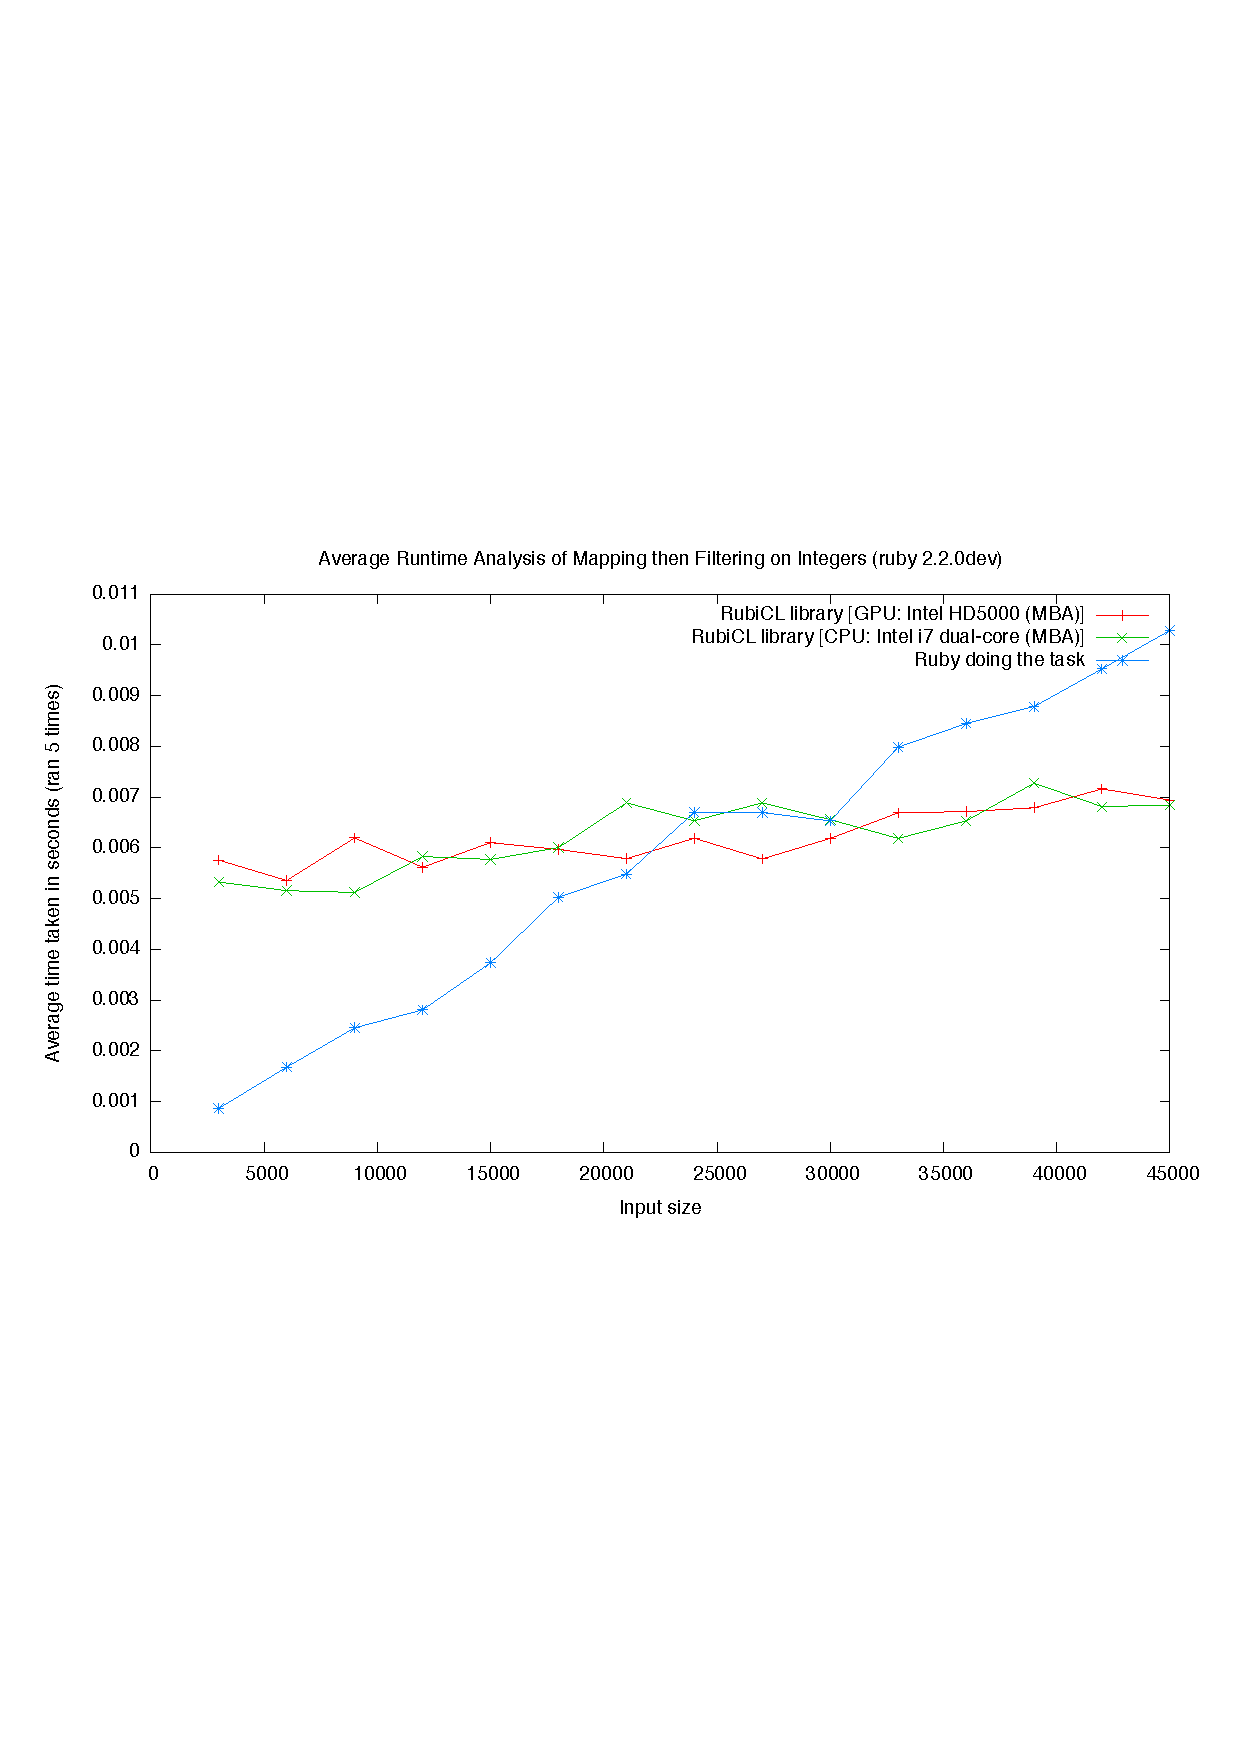
\includegraphics[trim=0cm 8cm 0cm 8cm, clip=true, width=\textwidth]{./graphing/smallmapfilter.pdf}
  \caption{Duration for smaller-scale \emph{MapFilter} tasks.}
  \label{fig:mapfil_tasksmallrun}
\end{figure}
Figure~\ref{fig:mapfil_tasksmallrun} shows that the RubiCL library, when executing on the laptop system, is beneficial for sparse \emph{MapFilter} tasks containing greater than $25,000$\textendash$30,000$ elements. It also demonstrates that the laptop system experiences task latency of around $50$ms.

\subsubsection{Floating-point performance}
\begin{figure}
  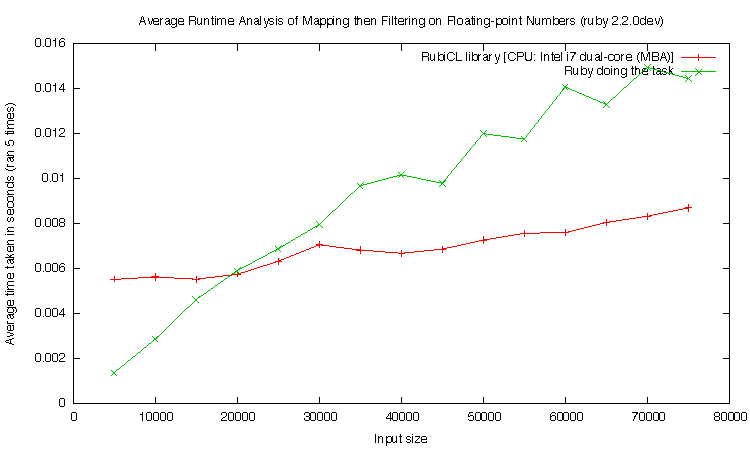
\includegraphics[width=\textwidth]{./graphing/dmapfilter.pdf}
  \caption{Duration for smaller-scale \emph{MapFilter} tasks on floating-point numbers}
  \label{fig:dmf_task_smallrun}
\end{figure}

\begin{figure}
  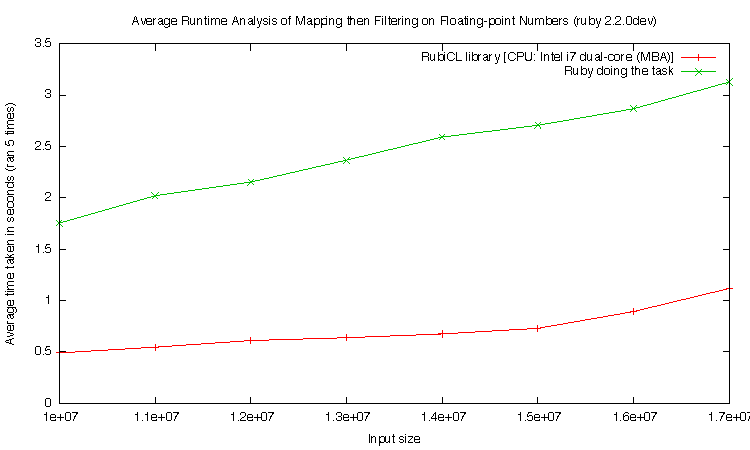
\includegraphics[width=\textwidth]{./graphing/dmapfilterlots.pdf}
  \caption{Duration for larger-scale \emph{MapFilter} tasks on floating-point numbers}
  \label{fig:dmf_task_bigrun}
\end{figure}

Figure~\ref{fig:dmf_task_smallrun} shows that the lower-bound for beneficial \emph{MapFilter} acceleration by the RubiCL library remains roughly the same for floating-point datasets as what was observed for integer datasets. Comparing \ac{OpenCL} execution on the \ac{CPU} to standard Ruby, it is worth outsourcing computation above $20,000$ elements, shown in Figure~\ref{fig:dmf_task_bigrun}.

The RubiCL library offers a speed-up of around $3$\textendash$4$ times the traditional implementation. This is nearly identical to the \ac{CPU} speed-up achieved for integer datasets and again suggests that the added cost of object dereferencing and re-creation is insignificant.



\subsection{Sort tasks}
\subsubsection{Integer performance}
\begin{figure}[H]
  \centering
  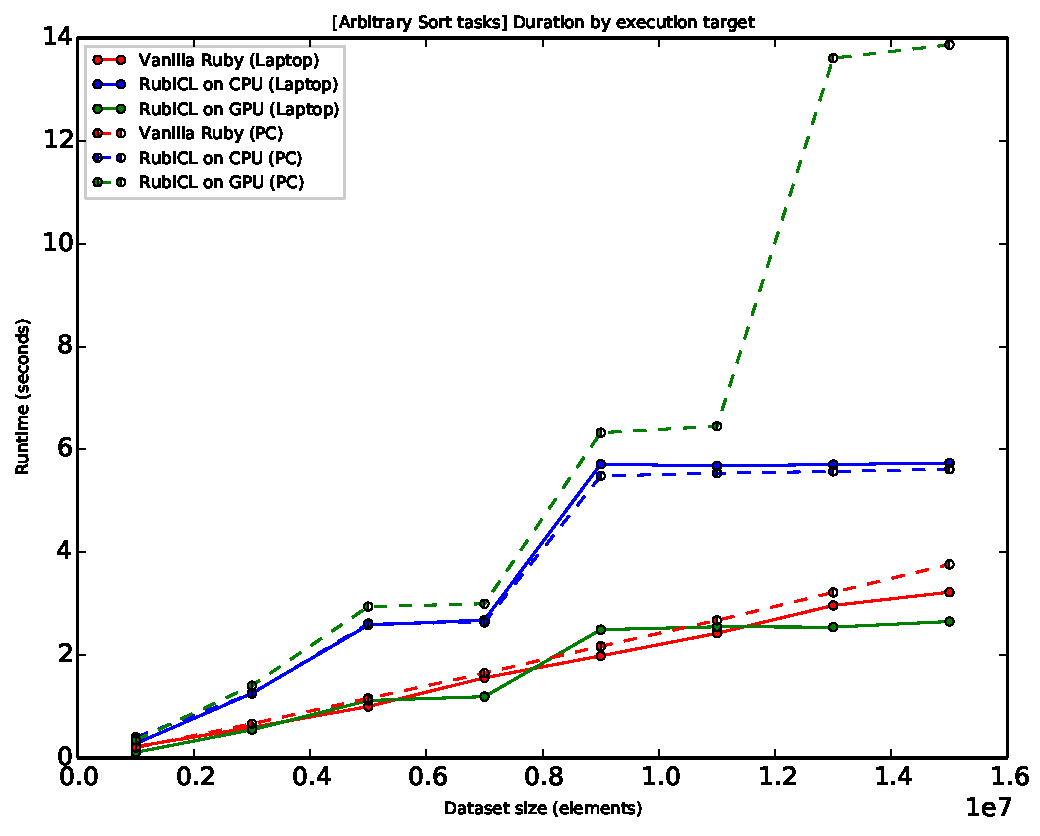
\includegraphics[width=\textwidth]{./graphing/sort_borked/runtimes.pdf}
  \caption{Task duration by execution target for sorting arbitrary datasets.}
  \label{fig:sortbork_task_runtime_g}

  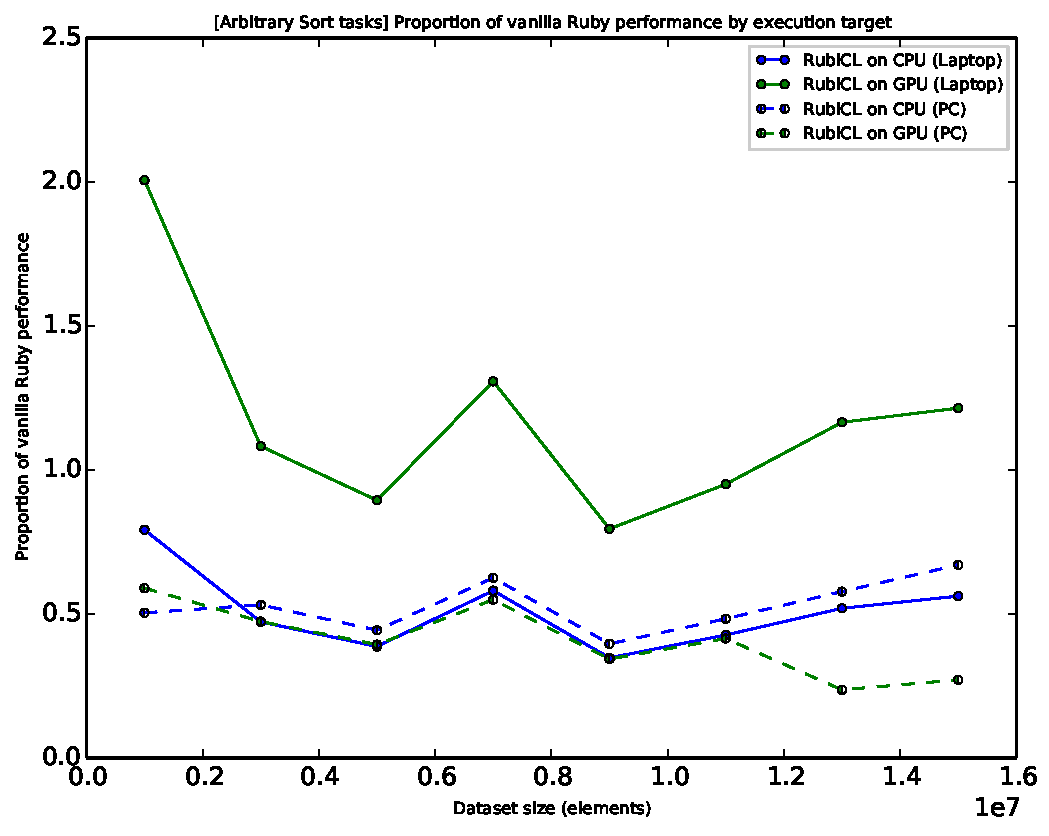
\includegraphics[width=\textwidth]{./graphing/sort_borked/prop_van.pdf}
  \caption{Proportion of vanilla Ruby performance achieved for sorting arbitrary datasets.}
  \label{fig:sortbork_van_perf_g}

\end{figure}

\begin{figure}[H]
  \centering
  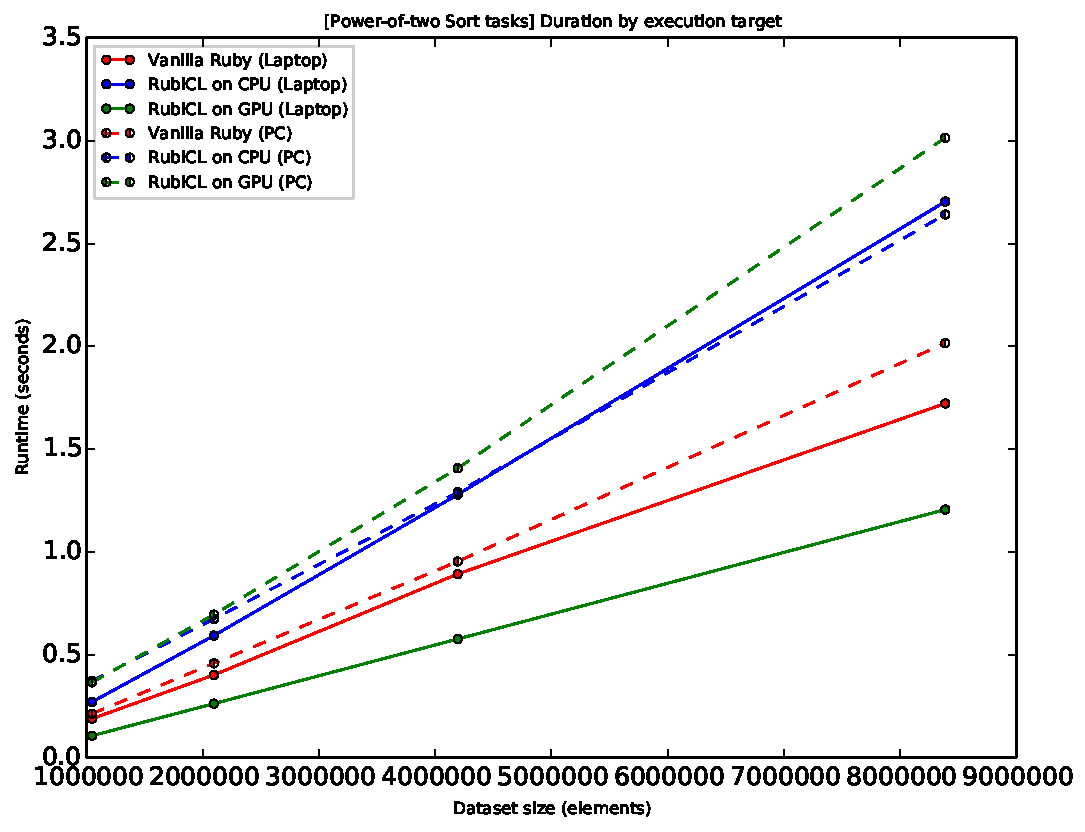
\includegraphics[width=\textwidth]{./graphing/sort_pow2/runtimes.pdf}
  \caption{Task duration by execution target for sorting power-of-two sized datasets.}
  \label{fig:sortpow_task_runtime_g}

  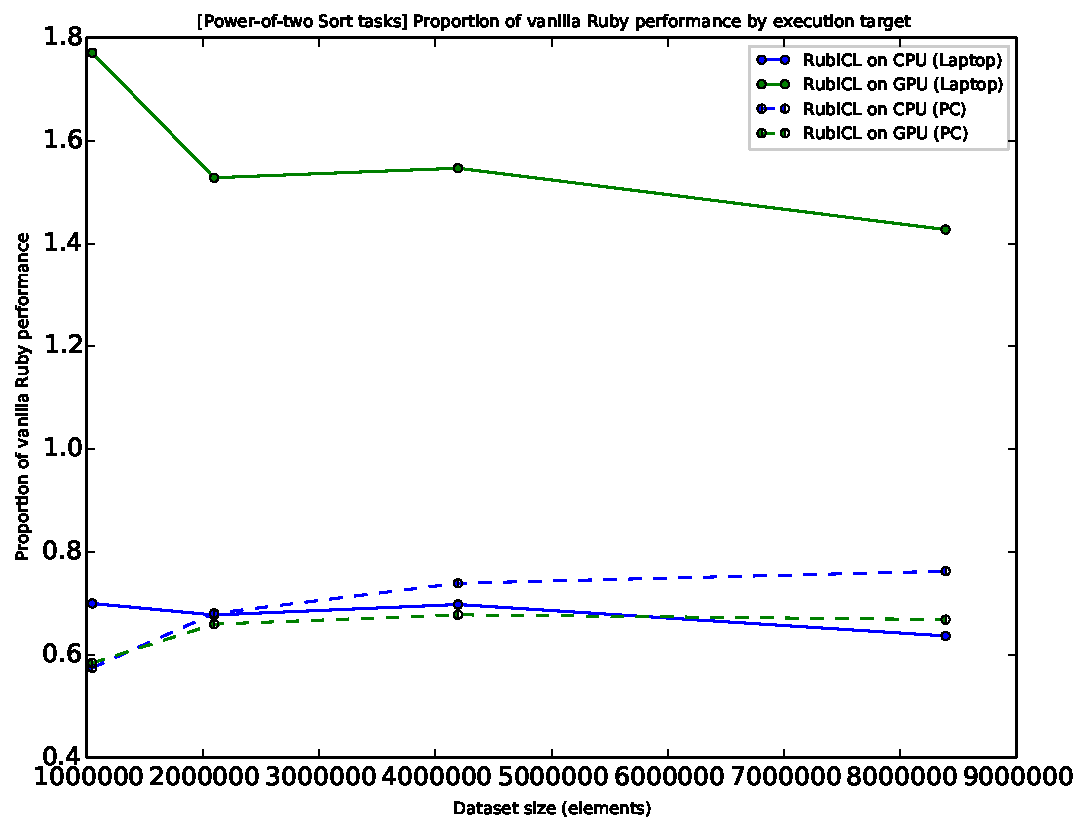
\includegraphics[width=\textwidth]{./graphing/sort_pow2/prop_van.pdf}
  \caption{Proportion of vanilla Ruby performance achieved for sorting power-of-two sizes datasets.}
  \label{fig:sortpow_van_perf_g}

\end{figure}

\subsubsection{Recap of operation performed}
The shuffled datasets were sorted in ascending order, by triggering the \verb|sort| method of the collection.
RubiCL's implementation of sorting uses parallel bitonic sort. Standard Ruby $2.2$ \verb|Enumerable|s rely on \emph{quicksort}.

\subsubsection{Observations and analysis}
Figure~\ref{fig:sortbork_task_runtime_g} highlights a critical flaw within RubiCL's \emph{Sort} task implementation.
Parallel bitonic sorting requires power-of-two sized datasets for the sorting network to operate correctly. In order to utilise the algorithm for general-sized sorting, the library pads the input dataset with \verb|MAX_INT| until the next power-of-two size.

The flaw present stems from an inefficient method of padding and unpadding the dataset. First, the input dataset is copied into the trailing segment of a larger buffer that has been prepended with padding. This is far less efficient than resizing the buffer and writing padding into the end segment, although it was unclear how this could be achieved using the \ac{OpenCL} \ac{API} at the time that the task was implemented. Finally, the dataset is extracted from the front segment of the buffer, as it can be assumed that all padding has propagated to the end. This action uses a buffer copy again, instead of the far more efficient method of returning a sub-buffer. All this unnecessary transfer of data produces an extraneous delay governed by memory bandwidth, and drastically decreases the performance for certain ratios of padding. The inefficient code was written in an attempt to implement the feature quickly and promptly forgotten about.

A large failing of the project in this regard was the fact that benchmarking of the sorting algorithm overlooked using non-power-of-two datasets. Due to the convenience of raising $2$ to a range of powers using the \verb|map| function, this method was used to generate seed sizes within the frequently used benchmarking scripts. Figure~\ref{fig:sortpow_task_runtime_g} shows that for power-of-two datasets, sort performance is not hindered. Therefore, the inefficiency was understandably missed.

Programming error aside, the performance of the sort algorithm on the \ac{CPU} of both systems is unsurprisingly lacking.
The \emph{compare-swap} bitonic sort algorithm used by RubiCL to perform sort tasks has $O(n \log^2 n)$ cost, greater than that of average-case \emph{quicksort}.
In addition, \emph{quicksort} is particularly celebrated for minimising the number of comparisons necessary to sort a dataset, resulting in far less work than \emph{bitonic mergesort}.
The increase in throughput provided by scheduling across many hardware threads of a \ac{CPU} was insufficient to offset having to perform a greater number of comparisons.

It is more interesting to note that Figure~\ref{fig:sortpow_van_perf_g} shows when sorting an integer dataset using the laptop's \ac{GPU}, performance around $1.5$ times that of inbuilt \emph{quicksort} can be achieved. It's important to realise that this does not mean \ac{GPU} sorting will triumph over \emph{quicksort} in other domains, though more efficient \ac{GPU} sorting algorithms have been shown to provide significant speed-up over \ac{CPU} sorting\cite{sintorn2008fast}. However, it is more likely in this case that a combination of no need for un-boxing variables within the RubiCL execution environment, combined with a still-strong sorting algorithm, resulted in the RubiCL implementation performing the task faster than the RubyVM could manage.

For some reason, the performance of the desktop \ac{GPU} was not as strong as that of the laptop \ac{GPU}. This is disappointing and further work should look into why this is the case.
\section{User evaluation}
\paragraph*{Recap of the study performed}
$7$ test-subjects were tasked with answering a test-file containing $5$ questions. Answers to questions were obtained by querying $2$ datasets of $10$ million elements each, with the assistance of the project's delivered library. This section presents the raw findings of the study, alongside interpretation and analysis.

\subsection{Results}
All applicants finished the $5$ question exercise within $20$ minutes. In most cases, the first question took the longest amount of time to complete, with an average of $4.5$ minutes. This can be explained by most people choosing to re-read the documentation and become accustomed with library usage before progressing. The next question was generally quicker to solve, with a mean of $3$ minutes, as it only involved applying a filtering stage to the previous counting pipeline. The third question took longer for most applicants, at a mean of $4$ minutes, as it introduced the new concepts of zipping and summation reduction. By the fourth question, subjects were more accustomed with the library's usage and it took a mean of $2$ minutes to complete. The final task was quick for most applicants also, taking a mean of $2.25$ minutes. In addition, most of the time was spent de-cyphering the complex requirements of the question.

\subsection{Test demographics}
The level of programming experience present in test subjects was as follows:
\begin{itemize}
    \item 3 applicants were final-year Informatics Master's students.
    \item 1 applicant was a final-year Informatics Bachelor student.
    \item 2 applicants were third-year Informatics Bachelor students.
    \item 1 applicant was a graduate of an unrelated discipline, with very little prior programming experience.
\end{itemize}

\paragraph*{Effect on performance}
In general, it was found that more-seasoned programmers completed the tasks sooner. Importantly though, this appeared not to be because those with less experience had difficulty. Instead, it appeared to be the case that experienced programmers could simply transcribe their thought processes into code faster, perhaps due to greater experience of thinking about execution whilst typing.

\subsection{Observations made}
\begin{itemize}
  \item A common theme throughout all test subjects: They avoided reading documentation as much as possible until they encountered difficulties and became stuck.
  This highlights the need to produce a library whereby experimentation can often yield the correct answer, as people are reluctant to have to read how something work instead of finding out for themselves.

  \item Forgetting to annotate a dataset with its type declaration was common for early questions. This was particularly true for subjects with prior experience of the Ruby programming language, perhaps due to the familiarity of the task causing them to write commonplace unannotated code without further thought. Luckily, this mistake became much less common after it had been made a couple of times. All subjects were less likely to make the same mistake repeatedly as the progressed through questions.

  \item Most people gave anonymous function parameters useless names, like $x$, when there was only one. In contrast, meaningful names, like $id, amount$, were used when there were several bound variables present.
    This justifies the project's decision to provide function parsing support, as it allows arbitrary naming of bound variables used within calculations by the programmer.

  \item Experienced programmers were more likely to state filtering predicates over several distinct pipeline stages, citing ease of readability as a motivating factor. This demonstrates the need to support \emph{task-fusion} within a pipeline-based execution environment. Otherwise, there would be an unnecessary penalty associated with orchestrating queries this way.

  \item There was confusion as to how zipping was achieved in the library, again this was particularly prevalent among experienced Ruby programmers. This was manifested as them attempting to zip datasets after both had been annotated, despite the documentation stating that only the first dataset needs to annotated and not the method argument. This was less common with subjects inexperienced with Ruby as they read the documentation first. This suggests that, in further work, the \verb|zip| method should be revisited and perhaps redesigned to be more explicit in usage.

  \item  When typos were made within parsed anonymous functions, subjects understood the error message provided. This occurred despite it mentioning ``method sending not implemented for \verb|$VARIABLE_NAME|'' whenever incorrectly written bound variable were interpreted as a function invocation request.

  \item The user with little programming experience did not find the library difficult to utilise or the questions hard to answer, after the process of stating computation as a pipeline of operators was explained. This suggests that the library may be suitable for analysts with little programming experience if they can quickly get to grips with how to orchestrate queries.

  \item Programmers with greater experience in the target language did a better job of highlighting inconsistent behaviour. For example, one user tried supplying a function argument to the \verb|count| operator, something that was unimplemented at the time as it had not been considered. This inconsistency was later fixed, but its discovery demonstrated the need for expert users in addition to novices when testing usability.

  \item There was no correlation between prior parallel programming ability and performance in the task. When questioned about levels of previous experience after the task, several participants stated they had no idea that the library was performing queries in parallel at all.

  \item There was no correlation between prior \ac{GPU} programming experience and task performance. Again, when questioned, no participants were aware that execution was occurring on the laptop \ac{GPU}.

\end{itemize}

\subsection{Solution performance}
Due to the questions being designed to only have one possible answering technique, all produced solutions took near-identical time to execute.
Each question restarted the computation pipeline instead of carrying on, in order to keep answers distinct and easier to reason about.

The mean time of execution, on the testing laptop's \ac{GPU}, for the produced solutions was $12.2$ seconds.
This compares favorably with the $49.5$ seconds required by an identical pure-Ruby implementation, giving a speed-up factor of $4.06$.

\section{Portability}
As mentioned during the \emph{Introduction} chapter, \ac{OpenCL} is still harder to utilise on some systems than the corresponding hardware vendors would have you believe.

On Apple hardware, such as the laptop used for development, achieving a working system is trivial.
The system comes with all dependencies required for \ac{OpenCL} \ac{GPGPU}. Utilising the library is as simple as remembering to include the correct header location. For some reason Apple decided that it should live at \verb|<OpenCL/opencl.h>|, while every other \ac{OS} presents the \ac{OpenCL} header at \verb|<CL/cl.h>|.

On the \ac{AMD} desktop system, operating \emph{Arch Linux}, installation of a complete set of working \ac{OpenCL} components was quite a bit more involved.
The \ac{OpenCL} framework uses a system, called \ac{ICD}, to allow many vendor-specific implementations of the library to be loaded on a single machine simultaneously.

Unfortunately, the root, vendor agnostic, \ac{ICD} loader is out of date in the \emph{Arch Linux} repositories, with only \ac{OpenCL} $1.1$ support. Luckily, it was possible to build \verb|libopencl|, provided by \ac{AMD}, from source and install the \ac{ICD} loader correctly.
Once the loader was installed, obtaining the actual \ac{ICD} component was straightforward, it is contained within the \ac{AMD} APP SDK, available in the \ac{AUR}.
However, the AMD APP SDK only provides \ac{CPU} drivers for \ac{OpenCL} execution. Furthermore, the default, \emph{free} \ac{AMD} display drivers do not allow \ac{OpenCL} access to onboard \ac{GPU} devices. The solution is to install the proprietary \verb|catalyst-utils| package, again from the \ac{AUR}. This provides required kernel modules for \ac{AMD} \ac{GPU} utilisation.

The final remaining issue is that \verb|catalyst-utils| only supports a significantly out of date version of \verb|xorg-server|. This could cause issues in a system used for daily activities, as dependency clashes could leave the user having to choose between \ac{OpenCL} support and the ability to run recently-developed desktop software.
